% =====================================================================
%  Massimizzazione dell'influenza con vincolo di diversità
%  su rete multistrato — relazione di progetto
%  Analisi di Social Network e Media · DIMES · Università della Calabria
%
%  Compilazione:  pdflatex relazione && bibtex relazione && pdflatex relazione && pdflatex relazione
%  Le figure stanno in figure/ e si rigenerano con figure.py e schemi.py.
%
% =====================================================================
\documentclass[11pt,a4paper]{article}

\usepackage[utf8]{inputenc}
\usepackage[T1]{fontenc}
\usepackage[italian]{babel}
\usepackage{lmodern}
\usepackage{microtype}
\usepackage[a4paper,margin=27mm]{geometry}
\usepackage{amsmath,amssymb}
\usepackage{graphicx}
\usepackage{booktabs}
\usepackage{array}
\usepackage{caption}
\usepackage{subcaption}
\usepackage{xcolor}
\usepackage{enumitem}
\usepackage[numbers,sort&compress]{natbib}
\usepackage[hidelinks]{hyperref}

\graphicspath{{figure/}}
\captionsetup{font=small,labelfont=bf,width=0.92\textwidth}
\setlist{nosep}

% -------------------------------------------------- comandi di comodo
\newcommand{\dascrivere}[1]{\textcolor{orange!80!black}{\textit{[da scrivere: #1]}}}
\newcommand{\Qtras}{Q_{\mathrm{tras}}}
\newcommand{\Qesp}{Q_{\mathrm{esp}}}
\newcommand{\phat}{\hat{p}}
\newcommand{\sx}{StackExchange}
\newcommand{\hg}{Higgs Twitter}
\newcommand{\num}[1]{#1}
% «dove siamo»: una riga di orientamento all'inizio di ogni fase
\newcommand{\dovesiamo}[4]{\par\noindent\begingroup\small\color{black!55}
  \textit{Dove siamo:} #1\\
  \textit{Ingresso:} #2\\
  \textit{Uscita:} #3\\
  \textit{Giudizio:} #4\par\endgroup\medskip}

\title{Massimizzazione dell'influenza con vincolo di diversità\\su rete multistrato\\[4pt]
  \large Dal cancello sul substrato alla previsione di chi adotterà}
\author{Davide Cinelli \qquad Giuseppe Cuiuri\\[10pt]
  \small Analisi di Social Network e Media \,·\, prof.~Andrea Tagarelli\\
  \small CdLM in Ingegneria Informatica \,·\, DIMES \,·\, Università della Calabria}
\date{Settembre 2026}

\begin{document}
\maketitle

\tableofcontents
\clearpage

% =====================================================================
\section{Introduzione}
\label{sec:intro}

\subsection{Il problema}
Qualcosa si diffonde su una rete sociale: un'idea, una notizia, una tecnologia. Chi osserva la rete prima che la diffusione esploda può porsi due domande. La prima è una domanda di previsione: \emph{chi adotterà?} La seconda è una domanda di ottimizzazione: \emph{da chi conviene partire}, se si vuole che adottino in molti e non in un solo angolo della rete? Tre strumenti dell'analisi delle reti parlano a entrambe: la \emph{community detection}, che trova i gruppi lungo cui la diffusione si incanala; le \emph{graph neural network}, che imparano dalla struttura; l'\emph{influence maximization}, che sceglie i nodi da cui partire. Questo lavoro li usa tutti e tre, su dati reali, e li mette alla prova l'uno contro l'altro.

La domanda iniziale era la seconda. Il progetto è nato come una pipeline di influence maximization con un vincolo di diversità su una rete multistrato, scegliere $k$ seed che massimizzino la diffusione toccando più comunità possibile, e la relazione racconta anche come, misurando, la domanda centrale sia diventata la prima.

\subsection{Perché è difficile: il modello che giudica sé stesso}
La difficoltà non sta negli algoritmi, che sono noti e hanno garanzie. Sta nel modo in cui vengono di solito valutati. Nella quasi totalità dei lavori di influence maximization le probabilità di trasmissione sugli archi sono \emph{assegnate} (una costante, o l'inverso del grado) e i seed scelti sotto quel modello sono valutati simulando lo stesso modello. Il ciclo si autoconferma: qualunque scelta risulti ottima è ottima rispetto a un'ipotesi che nessun dato ha verificato, e un risultato positivo non dice nulla sul mondo.

Il lavoro esce dal ciclo in due punti. Le probabilità si \emph{stimano} dai log di adozione, con la credit distribution e una GNN che la estende dove i log tacciono. E il giudizio finale si dà \emph{sui dati}: i seed si scelgono con ciò che si vede prima di un confine temporale, e si misura quanto indirizzano verso chi ha davvero adottato dopo. Nessuna simulazione decide chi ha ragione. Questa scelta ha un prezzo: i risultati possono essere negativi, e lo sono stati. Ed è il prezzo che rende gli altri credibili.

C'è una terza uscita, meno ovvia, che il lavoro ha dovuto costruire strada facendo: chiedersi \emph{prima} di tutto se la rete conti. Su un substrato in cui la diffusione non segue la topologia, ogni componente che usa la topologia misura rumore, e nessuna cura nel protocollo lo rivela. Il lavoro ha una misura per questo, l'eccesso strutturale contro un modello nullo a gradi preservati, e l'ha applicata con una soglia decisa in anticipo.

\subsection{Le due tesi}
\begin{enumerate}
  \item \textbf{Il substrato decide, e si può sapere prima.} Una misura da mezza giornata — l'eccesso strutturale stratificato contro un modello nullo a gradi preservati — predice se una pipeline di diffusione avrà qualcosa da trovare. Su \sx{} vale zero; su \hg{} vale $+73\%$.
  \item \textbf{Prevedere prima di ottimizzare.} L'ottimizzatore che massimizza \emph{quanti} nodi attiva perde contro il grado; quello che sa \emph{chi} adotterà lo batte. Le comunità sono il pezzo di conoscenza che pesa di più.
\end{enumerate}

\subsection{Contributi e struttura}
Il lavoro è stato eseguito per intero su due substrati: \sx{}, dove il progetto è nato, e \hg{}, dove è stato portato dopo che la misura del cancello ha dato esito opposto sui due. I suoi contributi sono i seguenti.
\begin{itemize}
  \item \textbf{Un cancello preregistrato sul substrato.} L'eccesso strutturale stratificato, con soglia fissata prima di misurare, ha detto no a \sx{} ($-0\%$) e sì a \hg{} ($+73\%$). \sx{} resta nel lavoro come controllo negativo: la prova che il protocollo sa dire di no.
  \item \textbf{Un criterio di Fase~1 fuori campione.} Le partizioni si giudicano sulla modularità della rete di trasmissione \emph{realizzata dopo il confine}, invece che su verità di riferimento contemporanee ai dati. Su questo criterio le comunità pre-annuncio spiegano il 74\% delle trasmissioni ($Q = 0{,}62$).
  \item \textbf{L'accoppiamento multistrato tarato dal dato.} La fusione dei livelli con la normalizzazione convenzionale perde il 24\% di modularità; con il peso degli strati scelto in campione, vince. Il verdetto sul multistrato dipende da una scelta che di solito non viene dichiarata.
  \item \textbf{La soglia di percolazione, localizzata, e la misura di non stazionarietà.} La rete di Higgs nel periodo calmo è sottocritica; l'annuncio del CERN moltiplica la trasmissività per 4,55 e la porta sopra soglia, che sta fra $\times 1{,}5$ e $\times 3$.
  \item \textbf{Il risultato negativo che ha cambiato il lavoro.} Sul criterio esterno il grado uscente batte TIM+ da $k = 20$ in su, e la GNN che stima $p$ l'86\% meglio della costante non produce seed migliori. Sapere \emph{come} si trasmette non aiuta a scegliere da chi partire.
  \item \textbf{Una scala di sette gradini per la previsione dell'adozione}, con cinque salti positivi sotto correzione di Bonferroni e bootstrap a grappoli sulle comunità. Le comunità sono la famiglia di attributi più informativa; la GNN aggiunge poco ma davvero; la struttura relazionale informa gli alberi ma non la GNN.
  \item \textbf{L'influence maximization pesata dalla previsione}, con probabilità out-of-fold, che batte il grado dell'11,85\% a $k = 10$ e del 7,06\% a $k = 20$, proprio dove il TIM+ non pesato perdeva, scegliendo utenti che non parlano ancora dell'evento.
\end{itemize}

La relazione segue l'ordine in cui il lavoro si capisce. Il capitolo~\ref{sec:background} raccoglie gli strumenti e dice dove ingannano. Il capitolo~\ref{sec:dati} descrive i due substrati e i loro limiti. Il capitolo~\ref{sec:sistema} presenta l'architettura e il pacchetto software. Il capitolo~\ref{sec:metodo} è la metodologia, fase per fase, e il capitolo~\ref{sec:protocollo} il protocollo sperimentale che decide che cosa conta come risultato. Il capitolo~\ref{sec:risultati} riporta i risultati nell'ordine in cui sono stati ottenuti, con i negativi accanto ai positivi; il capitolo~\ref{sec:discussione} li interpreta e ne fissa i limiti; il capitolo~\ref{sec:conclusioni} chiude. Il codice, le uscite di ogni esperimento, gli script delle figure e i comandi per riprodurre tutto sono nel repository del progetto.

% =====================================================================
\clearpage
\section{Background}
\label{sec:background}

Questo capitolo raccoglie gli strumenti che il lavoro usa, nell'ordine in cui compaiono nella pipeline. Non è una rassegna: di ciascuno si dice quello che serve a capire perché è stato scelto e dove può ingannare, e si rimanda alla Metodologia per come è stato applicato.

\subsection{Modelli di diffusione e soglia di percolazione}
Una diffusione su una rete si modella come un processo in cui i nodi passano da inattivi ad attivi lungo gli archi. Nel modello \emph{Independent Cascade} (IC) \citep{kempe2003} ogni nodo appena attivato tenta \emph{una volta sola} di attivare ciascun vicino uscente $v$, e riesce con probabilità $p(u,v)$; nel \emph{Linear Threshold} ogni nodo si attiva quando la somma dei pesi dei vicini attivi supera una soglia propria. Il lavoro usa IC, perché la credit distribution stima direttamente $p(u,v)$ e perché il campionamento a raggiungibilità inversa (sotto) è definito per IC.

Sotto IC la diffusione ha una \emph{soglia di percolazione}. In prima approssimazione conta il fattore di ramificazione (il numero atteso di attivazioni che un nodo attivo produce, cioè grado uscente per probabilità media), ma su reti con code di grado pesanti la quantità che decide è $\langle k^2 \rangle / \langle k \rangle$ moltiplicata per $p$, e può superare uno anche con $p$ molto piccola. Sopra soglia un solo seed raggiunge una componente gigante; sotto, ogni cascata si spegne. La conseguenza per l'influence maximization non è ovvia e la sezione~\ref{sec:met-fase2} la rende operativa: sopra soglia migliaia di nodi hanno copertura marginale equivalente, e qualunque confronto fra insiemi di seed misura rumore.

\paragraph{Che cosa percola.} Il termine viene dalla fisica dei mezzi porosi, e l'immagine è utile. Si lanci una moneta su ogni arco della rete: l'arco è \emph{vivo} con probabilità $p(u,v)$, \emph{morto} altrimenti. Gli archi vivi formano un sottografo casuale, e sotto Independent Cascade una cascata partita da un seed raggiunge esattamente i nodi che il seed raggiunge lungo gli archi vivi: tutto il resto della rete, per quella cascata, non esiste. Se le $p$ sono piccole gli archi vivi sono pochi, il sottografo è fatto di frammenti minuscoli, e una cascata partita da un nodo qualunque resta confinata nel suo frammento: si spegne dopo pochi passi. Crescendo le $p$, a un certo valore compare una \emph{componente gigante} di archi vivi, che attraversa una frazione macroscopica della rete: è la soglia di percolazione, e ciò che percola è l'attivazione. Sopra soglia, chiunque stia nella componente gigante raggiunge tutta la componente, e la scelta del seed smette di contare.

Nel lavoro il termometro è la dimensione degli insiemi RR (\S\ref{sec:bg-im}): un insieme RR è per costruzione il frammento di archi vivi raggiungibile all'indietro dalla radice, e la sua dimensione media dice da quale parte della soglia si sta, decine di nodi sotto, migliaia sopra. La Fase~2 usa questa misura per tarare il regime, e la sezione~\ref{sec:met-fase2} spiega come.

\subsection{Influence maximization: greedy, RR-sketch, TIM}
\label{sec:bg-im}
Il problema dell'\emph{influence maximization} \citep{kempe2003} è scegliere $k$ nodi seme che massimizzino la diffusione attesa $\sigma(S)$ sotto il modello. È NP-hard \citep{kempe2003}, ma $\sigma$ è monotona e sottomodulare (aggiungere un seme a un insieme piccolo rende più che aggiungerlo a un insieme grande) e per le funzioni sottomodulari il greedy che a ogni passo prende il nodo con il massimo guadagno marginale ottiene almeno $(1 - 1/e) \approx 0{,}63$ dell'ottimo. Il collo di bottiglia è valutare $\sigma$, che è \#P-difficile e si stima per simulazione: il greedy originale con Monte Carlo costa $O(k \cdot n \cdot r \cdot m)$ e non scala.

Il campionamento a \emph{raggiungibilità inversa} \citep{borgs2014} capovolge il problema. Si estrae un nodo $v$ a caso, si genera una realizzazione del grafo in cui ogni arco è vivo con la propria probabilità, e si raccoglie l'insieme dei nodi da cui $v$ è raggiungibile \emph{all'indietro}: l'insieme RR di $v$, cioè chi avrebbe potuto attivarlo. Il teorema che regge tutto è che $\sigma(S)$ è proporzionale alla probabilità che un insieme RR intersechi $S$: massimizzare la diffusione diventa quindi \emph{massima copertura} di una collezione di insiemi, che è di nuovo sottomodulare e che il greedy risolve in tempo lineare nella dimensione della collezione (figura~\ref{fig:rr}). TIM e TIM+ \citep{tang2014} rendono il metodo pratico stimando quanti insiemi servono per una garanzia $(1 - 1/e - \varepsilon)$. Il lavoro usa 120.000 insiemi per configurazione, un numero fissato a priori e tenuto in cache, e valuta la stabilità della scelta ripetendo il campionamento con un altro seme.

Un'estensione che il capitolo finale usa: se le radici degli insiemi RR non si estraggono uniformemente ma in proporzione a un peso $w(v)$, la copertura stima la somma dei pesi dei nodi attivati invece del loro numero \citep{borgs2014}. È l'influence maximization \emph{pesata sui nodi}, e il greedy non cambia.

\begin{figure}[htbp]
  \centering
  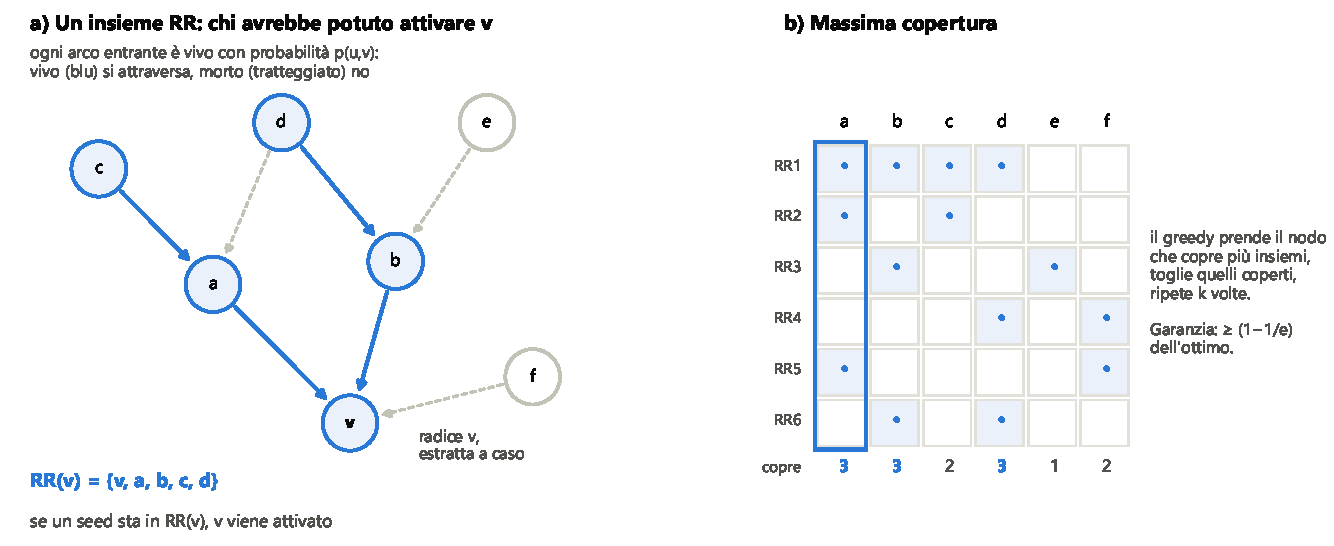
\includegraphics[width=\textwidth]{schema_rr}
  \caption{Un insieme RR e la massima copertura. (a)~Si estrae una radice $v$ e si visita il grafo \emph{all'indietro}, attraversando ogni arco entrante con probabilità $p(u,v)$: l'insieme raggiunto è chi avrebbe potuto attivare $v$. (b)~La diffusione attesa di un insieme di seed è proporzionale alla frazione di insiemi RR che interseca; il greedy sceglie ogni volta il nodo che copre più insiemi ancora scoperti, con garanzia $1-1/e$.}
  \label{fig:rr}
\end{figure}

\subsection{Diversità: il vincolo di DTIM}
\label{sec:bg-dtim}
Il vincolo cambia una sola espressione nel criterio di scelta del greedy:
\begin{equation}
  s(v) \;=\; \alpha \cdot \frac{|R_v|}{\max_u |R_u|} \;+\; (1-\alpha)\cdot \mathbf{1}\big[\,c(v)\notin C\,\big],
  \label{eq:dtim}
\end{equation}
dove $|R_v|$ è il numero di insiemi RR non ancora coperti da un seed già scelto che contengono $v$, $c(v)$ è la comunità di $v$ e $C$ è l'insieme delle comunità in cui sta già almeno un seed. Con $\alpha=1$ si riottiene TIM+ esatto: la baseline non è un'altra implementazione da confrontare, è lo stesso codice con un parametro diverso.

Il greedy lavora a passi. Al passo $j$ ha già scelto $j-1$ seed, calcola $s(v)$ per ogni candidato $v$ e prende il massimo. Il primo termine è la \emph{copertura marginale} di $v$: $|R_v|$ conta quanti insiemi RR $v$ coprirebbe in più se venisse aggiunto, cioè, per il teorema della raggiungibilità inversa, quanto aumenterebbe la diffusione attesa. Non è un numero fisso, perché ogni seed scelto toglie dal conto gli insiemi che copre, e $|R_v|$ cala per tutti i nodi che li condividevano. La divisione per $\max_u |R_u|$, il guadagno del candidato migliore a quel passo, porta il termine in $[0,1]$: vale 1 per chi copre di più, 0,5 per chi ne copre la metà. Il secondo termine è il \emph{premio di diversità}: l'indicatore vale 1 se la comunità di $v$ non ha ancora nessun seed e 0 altrimenti, ed è un bonus fisso a chi apre una comunità nuova. Il peso $\alpha$ regola quanto il premio conta rispetto alla copertura. Scelto il seed, si aggiorna lo stato: i suoi insiemi RR escono dal conto e la sua comunità entra in $C$; quando tutte le comunità premiabili sono in $C$, il premio vale zero per tutti e il greedy torna a essere TIM+ puro sui seed che restano.

Due proprietà della formula non sono cosmetiche. La \emph{normalizzazione sul massimo} è necessaria: senza, i conteggi di copertura valgono centinaia e schiaccerebbero un indicatore che vale 0 o 1, e $\alpha$ non avrebbe alcun effetto. E il \emph{tasso di scambio} è $(1-\alpha)/\alpha$: un nodo in una comunità già toccata batte uno che ne apre una nuova solo se la sua copertura normalizzata supera l'altra di almeno quella quantità. Poiché la copertura normalizzata sta in $[0, 1]$, per $\alpha \le 0{,}5$ il vantaggio richiesto è $\ge 1$ e quindi irraggiungibile: sotto quella soglia la diversità domina in modo assoluto e ogni seed apre necessariamente una comunità nuova finché ce ne sono. È una previsione della formula, e i risultati la confermano (figura~\ref{fig:superficie}: a $\alpha = 0{,}5$ e $\alpha = 0{,}3$ le celle coincidono). Il criterio è quello del Diversity-aware TIM (DTIM) di \citet{calio2018}; il lavoro vi aggiunge una soglia di dimensione sulle comunità premiabili, per la ragione detta in \S\ref{sec:met-fase3}.

\subsection{Community detection e reti multistrato}
La \emph{modularità} \citep{newman2006} misura quanto una partizione concentra gli archi dentro le comunità rispetto a quanto ci si aspetterebbe da una rete casuale con la stessa sequenza di gradi:
\begin{equation}
  Q \;=\; \frac{1}{2m} \sum_{u,v} \Big[ A_{uv} - \frac{k_u k_v}{2m} \Big]\, \delta(c_u, c_v),
  \label{eq:modularita}
\end{equation}
con $A$ l'adiacenza pesata, $k_u$ il grado di $u$, $m$ il peso totale e $\delta$ che vale 1 se i due nodi stanno nella stessa comunità. Il termine sottratto, $k_u k_v / 2m$, è il modello nullo a gradi preservati (sotto): la modularità non è «quanti archi sono interni» ma «quanti più di quanti ce ne sarebbero per caso», ed è questo che la rende adatta a giudicare partizioni senza premiare quelle degeneri. Vale circa zero sia per la partizione unica sia per quella a singoletti.

\emph{Louvain} \citep{blondel2008} massimizza $Q$ per spostamenti locali e aggregazione ripetuta, ed è lo standard per reti grandi. Ha un difetto noto: può produrre comunità \emph{internamente sconnesse}, perché lo spostamento di un nodo può tagliare in due la comunità che lascia senza che l'algoritmo se ne accorga. \emph{Leiden} \citep{traag2019} aggiunge una fase di raffinamento che garantisce comunità connesse a ogni livello. Nel lavoro la garanzia ha un senso preciso. Nella Fase~3 il vincolo di diversità considera una comunità «coperta» appena contiene un seed, nell'ipotesi che da quel seed l'influenza possa raggiungere il resto della comunità. Se la comunità è fatta di due pezzi non collegati fra loro, un seed nel primo pezzo la fa contare come coperta ma non può raggiungere il secondo: il vincolo crede di aver aperto una comunità e in realtà ne ha aperta metà. Comunità connesse evitano questo caso. I risultati mostrano però che sul criterio decisionale i due algoritmi sono indistinguibili (\S\ref{sec:risultati}).

Una rete \emph{multistrato} ha più tipi di relazione fra gli stessi nodi: qui risposte e commenti su \sx{}, follow, retweet, mention e reply su \hg{}. Il modo più semplice di usarla è fondere i livelli in una rete sola, pesando ciascuno; la scelta dei pesi è una decisione che di solito non viene dichiarata, e il lavoro mostra che decide il verdetto (\S\ref{sec:met-fase1}). L'alternativa è il \emph{consenso di ensemble}: M-EMCD \citep{tagarelli2017} calcola una partizione per livello e ne cerca una che le rappresenti tutte, con un parametro $\theta$ che regola quanto le partizioni di livello devono concordare. È stato provato sulla prima versione del progetto, su \sx{}, e riportato in appendice~\ref{app:stackexchange}.

\subsection{Valutare una partizione: NMI, AMI, modello nullo}
Confrontare una partizione con una verità di riferimento sembra un problema risolto dall'\emph{informazione mutua normalizzata} (NMI), e non lo è. L'NMI non è corretta per il caso: due partizioni indipendenti hanno informazione mutua positiva, che cresce col numero di cluster, e l'NMI la conta come accordo. Il risultato è che l'NMI premia la granularità come se fosse accuratezza, fino al caso limite della partizione a singoletti, che prende un punteggio alto senza dire nulla. L'\emph{informazione mutua aggiustata} (AMI) \citep{vinh2010} sottrae il valore atteso sotto assegnazione casuale a cluster delle stesse dimensioni, e per la partizione a singoletti vale zero. Il lavoro riporta entrambe su un controllo degenere, su due substrati, e la differenza è la misura di quanto l'NMI inganna (figura~\ref{fig:nmi}).

Lo stesso principio vale per giudicare se una rete «conta». Il \emph{modello nullo a gradi preservati} \citep{maslov2002} è la rete ricablata a caso tenendo fisso il numero di vicini di ogni nodo: ciò che sopravvive al ricablaggio è dovuto ai gradi, ciò che non sopravvive è dovuto alla topologia specifica. È il confronto che il cancello (\S\ref{sec:met-cancello}) fa esplicitamente, e che la modularità fa implicitamente dentro la propria definizione. Le metriche che non lo fanno (per esempio il rapporto fra archi intra-comunità osservati e attesi sotto un'assegnazione casuale che ignora i gradi) esplodono sulle partizioni quasi degeneri, e il lavoro le riporta solo per mostrarlo.

\subsection{GNN su grafi grandi}
Una \emph{graph neural network} produce per ogni nodo una rappresentazione che dipende dai suoi attributi e da quelli del vicinato, aggregati lungo gli archi. In \emph{GraphSAGE} \citep{hamilton2017} lo strato $\ell$ aggrega prima il vicinato e poi lo combina con la rappresentazione del nodo:
\begin{align}
  h^{(\ell)}_{N(v)} &= \operatorname{AGG}_\ell\big(\{\, h^{(\ell-1)}_u : u \in N(v) \,\}\big), \\
  h^{(\ell)}_v &= \sigma\big( W_{\mathrm{self}}^{(\ell)}\, h^{(\ell-1)}_v + W_{\mathrm{neigh}}^{(\ell)}\, h^{(\ell)}_{N(v)} \big),
  \label{eq:sage}
\end{align}
con $h^{(0)}_v = x_v$ gli attributi iniziali, $\sigma$ una non-linearità (qui ReLU) e $\operatorname{AGG}$ l'aggregatore, che nel lavoro è la media. Con $\ell = 1, 2$ la rappresentazione finale $h^{(2)}_v$ dipende dal vicinato a distanza due. Nel lavoro la GraphSAGE compare due volte: sugli \emph{archi}, per estendere la stima di $p(u,v)$ dove il log tace, con una \emph{testa} (lo strato finale, che dalla coppia di rappresentazioni $(h_u, h_v)$ produce il numero $p(u,v)$), e sui \emph{nodi}, come classificatore dell'adozione.

Il problema è la scala. A batch pieno ogni epoca richiede due prodotti fra l'adiacenza sparsa e la matrice degli attributi, in avanti e all'indietro, e su 456.627 nodi e 25 milioni di elementi non nulli costa decine di secondi; con centinaia di epoche e più semi diventa impraticabile su CPU. Due osservazioni lo risolvono. La prima è che nel primo strato il prodotto $A x$ non dipende dai pesi e si può calcolare una volta: è una riscrittura esatta. La seconda, più radicale, è di \emph{SGC} \citep{wu2019} e \emph{SIGN} \citep{frasca2020}: se si toglie la non-linearità fra un'aggregazione e l'altra, l'intera propagazione $[x, \tilde{A} x, \tilde{A}^2 x, \ldots]$ diventa un precalcolo, e il modello che segue, un MLP, lavora su una matrice densa e si addestra a mini-batch, in minuti invece che in ore, senza tenere il grafo in memoria. Si perde qualcosa in espressività, e il lavoro misura quanto: il confronto fra gli attributi propagati dati a un modello ad alberi e dati a un MLP isola il contributo della non-linearità.

Le reti \emph{relazionali}, R-GCN \citep{schlichtkrull2018}, estendono l'aggregazione a grafi con più tipi di arco, con una matrice di pesi $W_r$ per relazione: $h_v' = \sigma\big(W_0 h_v + \sum_r \sum_{u \in N_r(v)} \frac{1}{|N_r(v)|} W_r h_u\big)$. Un R-GCN a batch pieno ha lo stesso problema di scala della GraphSAGE, moltiplicato per il numero di relazioni; la sua versione con propagazione precalcolata, un operatore per relazione, una proiezione per operatore, poi la non-linearità, è il primo strato di un R-GCN nello spirito di SIGN, ed è quella che il lavoro usa e chiama R-SIGN.

\subsection{Stimare le probabilità: credit distribution}
Nella quasi totalità dei lavori di influence maximization le probabilità sugli archi sono \emph{assegnate}: una costante, oppure $1/\text{grado}$ del nodo di arrivo, oppure un valore estratto a caso da un insieme fisso. Il guaio non è l'approssimazione: è che l'insieme dei seed dipende da quei numeri, e la valutazione si fa poi simulando con gli stessi numeri. Il ciclo si autoconferma e non ha validità esterna.

La \emph{credit distribution} di \citet{goyal2010} stima $p$ dai log di azioni. Nella variante statica di Bernoulli, se $A(u)$ sono le azioni compiute da $u$ e $A(u \to v)$ quelle fra esse che $v$ ha ripetuto dopo, allora $p(u \to v) = A(u \to v) / A(u)$: di tutto quello che ha fatto $u$, quale frazione $v$ ha poi fatto? È una stima di correlazione temporale, non di causalità (due vicini possono adottare la stessa cosa perché rispondono entrambi a una tendenza esterna) e nessuna variante lo distingue; è esattamente ciò che il confronto col modello nullo delimita. Due cose la rendono utilizzabile in pratica. Uno smoothing $s$ al denominatore, che impedisce a un utente con una sola azione copiata una volta di ottenere $p = 1$: senza, sul primo substrato il 99° percentile di $p$ era esattamente uno, e la cascata simulata era sopra soglia. E una definizione del numeratore adatta al dato: su \sx{} è una coincidenza di adozioni, su \hg{} è un retweet osservato, e la differenza si vede nella qualità della stima (\S\ref{sec:risultati}).

% =====================================================================
\clearpage
\section{Dati}
\label{sec:dati}

Il lavoro usa due dataset che rappresentano due situazioni opposte, e la differenza fra i due è il primo risultato della relazione (\S\ref{sec:ris-cancello}). Entrambi hanno la stessa forma astratta: una rete relazionale osservabile \emph{prima} di un confine temporale, e un insieme di adozioni datate che si vogliono prevedere \emph{dopo}. Tutto ciò che i modelli vedono sta prima del confine; tutto ciò su cui vengono giudicati sta dopo. La tabella~\ref{tab:substrati} li mette a confronto.

\subsection{StackExchange}
Il primo substrato è il sito Security di StackExchange, dal dump pubblico dell'Internet Archive. È una comunità di domande e risposte su temi di sicurezza informatica, attiva dal 2010, in cui ogni domanda porta fino a cinque \emph{tag} che ne dichiarano l'argomento. Il primo uso di un tag da parte di un utente, come autore di una domanda o di una risposta, è un'\emph{adozione} datata al mese, e la sequenza delle adozioni di un tag fra gli utenti ricostruisce una diffusione realmente avvenuta: 319.697 eventi in tutto. Un'\emph{esposizione} è la coppia (arco, tag): $u \to w$ è un'esposizione per il tag $t$ se $w$ ha adottato $t$ dopo che $u$, suo vicino nella rete, lo aveva già adottato. È l'analogo, su questo substrato, della trasmissione realizzata di \hg{}, e la rete delle esposizioni dei tag bersaglio (64.711 archi) è il criterio $\Qesp$ con cui la Fase~1 era giudicata qui (appendice~\ref{app:stackexchange}).

La rete ha due livelli, entrambi orientati e pesati con il numero di interazioni:
\begin{itemize}
  \item \textbf{L1, risposta}: arco $u \to v$ se $u$ ha risposto a una domanda di $v$. È un atto tematico: si risponde su ciò che si sa.
  \item \textbf{L2, commento}: arco $u \to v$ se $u$ ha commentato un post di $v$. È un atto sociale: si commenta chi si segue.
\end{itemize}
I due livelli condividono lo stesso insieme di 46.312 nodi, unione degli estremi, con 88.318 archi in L1 e 138.767 in L2. Il confine temporale è il gennaio 2020: la rete e ogni stima usano solo eventi precedenti, la finestra di verifica è il 2020--2022. I \emph{tag bersaglio}, quelli la cui adozione si vuole prevedere, sono i 105 con almeno cento adozioni dopo il confine, e sono esclusi per costruzione sia dalla rete sia dalla stima delle probabilità: senza questa maschera lo stesso segnale costruirebbe la rete, definirebbe la verità di riferimento e sarebbe l'oggetto della previsione, e il progetto misurerebbe sé stesso. Confine e bersagli sono definiti in un solo modulo del pacchetto, da cui ogni altro modulo importa.

Un secondo sito, Computer Graphics (1.653 nodi, 26 tag bersaglio), è stato usato come replica su scala ridotta nella prima versione del progetto; i suoi numeri sono riportati in appendice~\ref{app:stackexchange}.

Nella finestra di verifica l'attività del sito principale scende da 889 a 467 utenti attivi al mese ($-48\%$ in tre anni). Il declino non contamina i confronti fra strategie, che sono appaiati e si fanno a parità di tag e di mese, ma va tenuto presente nel leggere i valori assoluti.

\subsection{Higgs Twitter}
Il secondo substrato è il dataset raccolto da \citet{dedomenico2013} attorno all'annuncio della scoperta del bosone di Higgs, disponibile su SNAP \citep{snap}. Copre sette giorni, dal 1° al 7 luglio 2012, e contiene due cose distinte:
\begin{itemize}
  \item il \textbf{grafo dei follower}: 456.627 utenti e 14.855.842 archi orientati, $A \to B$ se $A$ segue $B$;
  \item il \textbf{log delle attività}: 563.069 eventi datati al secondo, ciascuno della forma «$a$ ha ritwittato / menzionato / risposto a $b$» (RT, MT, RE).
\end{itemize}
L'\emph{adozione} di un utente è il primo istante in cui compare nel log, in qualunque ruolo: chi viene ritwittato era già nella conversazione, e i tweet originali non sono nel dataset. Ne compaiono 304.691 sui 456.627; gli altri 151.936 non adottano mai, e restano nel conteggio perché toglierli falserebbe verso l'alto ogni probabilità di adozione.

La rete ha quattro livelli. Il primo è il grafo dei follower, \textbf{F}: è il \emph{canale}, l'unico livello esogeno: esiste prima dell'evento e non è fatto di eventi di diffusione. Gli altri tre sono costruiti dal log, con i soli eventi precedenti al confine: \textbf{RT} (29.444 archi), \textbf{MT} (16.902) e \textbf{RE} (3.262). RE risulta interamente contenuto in MT (ogni reply è anche una mention) e va letto come un raffinamento di peso, non come una relazione indipendente. Tutti gli archi sono memorizzati nel verso in cui \emph{scorre l'influenza}: se $A$ segue $B$ l'arco è $B \to A$, se $a$ ritwitta $b$ l'arco è $b \to a$. La Fase~2 stima $p(u,v)$ come probabilità che $u$ attivi $v$, e quel verso deve essere quello giusto fin dall'inizio.

Il confine è all'\textbf{ora 72}, la mezzanotte UTC fra il 3 e il 4 luglio: poche ore prima dell'annuncio del CERN, che cade attorno all'ora 76, con il picco di 19.885 nuove adozioni all'ora 78 (figura~\ref{fig:adozioni}). Prima del confine hanno adottato 35.610 utenti; dopo, nelle 96 ore restanti, 269.081. È la domanda che l'influence maximization pone davvero: scegliere i seed quando l'evento non è ancora esploso, e vedere chi si attiva.

Un fatto del dato che pesa sul metodo: il 37\% delle trasmissioni osservate prima del confine (16.868 su 45.366) avviene fra utenti \emph{non} collegati da un arco di follow. Si ritwitta anche chi non si segue (attraverso le timeline altrui, la ricerca, i trend) e quella parte della diffusione non è modellabile su questo canale.

\subsection{Un limite da dichiarare}
Il grafo dei follower è stato raccolto \emph{attorno} all'evento, non prima: può contenere legami nati durante l'esplosione, e in quel caso una parte della struttura che la pipeline usa per prevedere sarebbe in realtà una conseguenza di ciò che deve prevedere. Con i dati disponibili non è correggibile (gli archi di follow non hanno data) e va scritto accanto a ogni risultato che usa il grafo. Un secondo limite è che il dataset contiene un evento solo: ogni bootstrap ricampiona unità \emph{dentro} l'evento (ore, comunità), mai eventi diversi.

Si fa presente infine una scelta che va considerata con attenzione. Usare la rete di retweet come substrato, che sarebbe la scelta più immediata, produce un test degenere: lì l'arco \emph{è} l'evento di diffusione, quindi nessun nodo può essere esposto prima di adottare, e la curva dose-risposta ha un punto solo. Serve un substrato che esista prima dell'evento, con la cascata che lo attraversa. Su StackExchange la separazione fra rete e adozioni c'era già; su Twitter va costruita, ed è il grafo dei follower.

\begin{table}[htbp]
  \centering\small
  \caption{I due substrati affiancati. «Verità vista in Fase 1»: su \sx{} la verità tematica per l'AMI copriva il 10\% dei nodi; su \hg{} il 97\% degli adottanti ha almeno una trasmissione osservata. L'ultima riga è la misura del cancello (\S\ref{sec:met-cancello}, \S\ref{sec:ris-cancello}).}
  \label{tab:substrati}
  \setlength{\tabcolsep}{4pt}
  \begin{tabular}{lll}
    \toprule
     & \sx{} (controllo negativo) & \hg{} (substrato di lavoro) \\
    \midrule
    canale & risposte e commenti & grafo dei follower \\
    nodi & 46.312 & 456.627 \\
    archi & 230.641 & 14.855.842 \\
    livelli & 2 & 4 — follower, retweet, mention, reply \\
    oggetto della diffusione & 105 tag tecnici, 12 anni & un evento, 7 giorni \\
    confine temporale & gennaio 2020 & ora 72 — 3 luglio 2012, notte \\
    da prevedere & 64.711 esposizioni & 269.081 adottanti \\
    verità vista in Fase 1 & 10\% dei nodi & 97\% dei bersagli \\
    \textbf{eccesso strutturale} & $\mathbf{-0\%}$ & $\mathbf{+73\%}$ \\
    \bottomrule
  \end{tabular}
\end{table}

\begin{figure}[htbp]
  \centering
  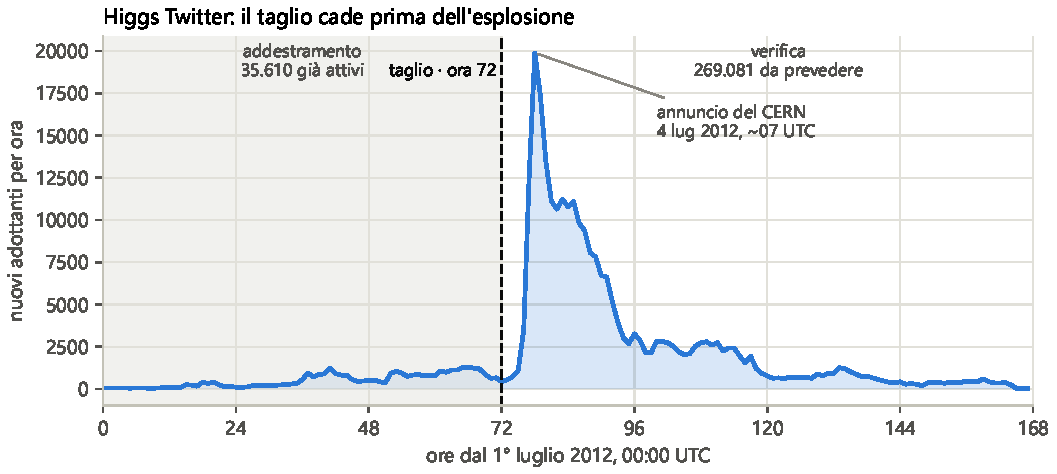
\includegraphics[width=\textwidth]{fig_adozioni_ora}
  \caption{Nuovi adottanti per ora su \hg{}. Il taglio all'ora 72 cade poche ore prima dell'annuncio del CERN: 35.610 utenti hanno già adottato, 269.081 adotteranno nelle 96 ore successive, 151.936 mai. Tutto ciò che i modelli vedono è a sinistra della linea.}
  \label{fig:adozioni}
\end{figure}

% =====================================================================
\clearpage
\section{Il sistema}
\label{sec:sistema}

\subsection{Architettura}
\begin{figure}[htbp]
  \centering
  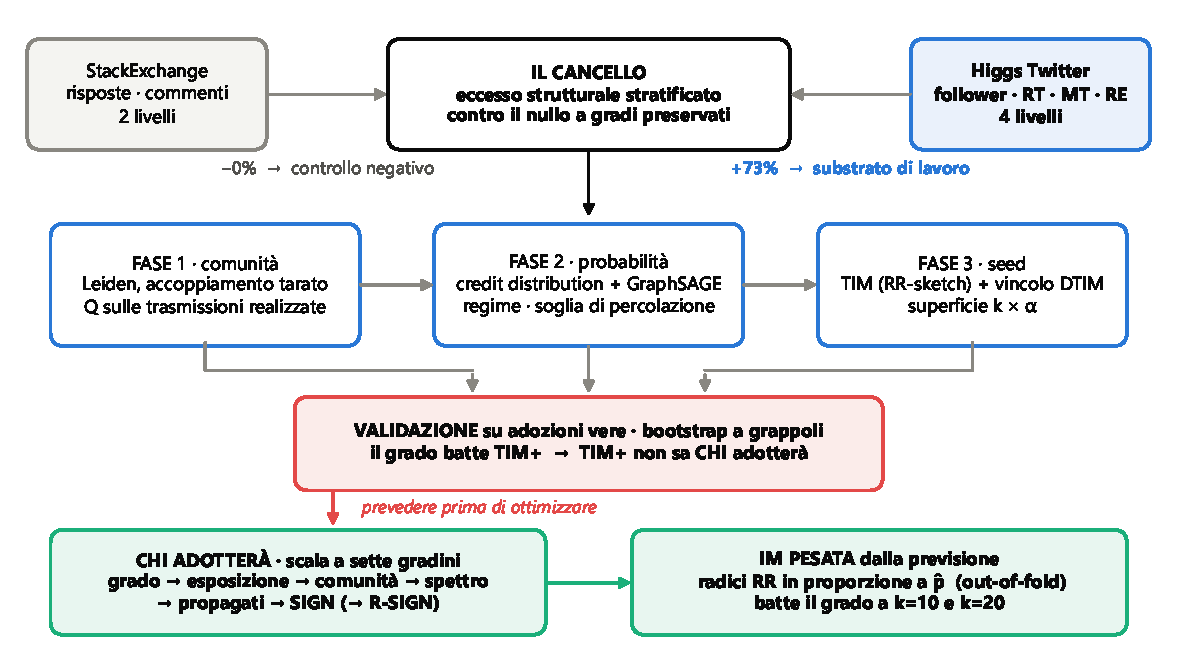
\includegraphics[width=\textwidth]{fig_architettura}
  \caption{L'architettura. Il cancello decide il substrato; le tre fasi producono comunità, probabilità e seed; la validazione su adozioni vere giudica — e dice che TIM+ non sa chi adotterà. Da lì il giro: la previsione dell'adozione e l'IM pesata dalla previsione.}
  \label{fig:architettura}
\end{figure}
La figura~\ref{fig:architettura} si legge dall'alto in basso, e l'ordine è quello in cui il lavoro è stato fatto.

In cima stanno i due substrati e, fra loro, il \textbf{cancello}: la misura dell'eccesso strutturale che decide se un substrato porta la diffusione. \sx{} entra come controllo negativo, \hg{} come substrato di lavoro. Sotto, le \textbf{tre fasi} della pipeline, ciascuna con un ingresso, un'uscita e un criterio di verifica proprio: la Fase~1 prende i livelli della rete e produce una partizione, giudicata sulle trasmissioni realizzate fuori campione; la Fase~2 prende i livelli e il log e produce una matrice $p$ di probabilità di trasmissione, con la sua taratura di regime; la Fase~3 prende $p$ e la partizione e produce gli insiemi di seed, per ogni budget $k$ e ogni peso $\alpha$ del vincolo di diversità. Ognuna alimenta la successiva, ma nessuna la giudica: il giudizio è il blocco sotto, la \textbf{validazione} sulle adozioni vere, che è l'unico posto in cui la finestra dopo il confine viene letta.

La validazione produce il risultato che ha cambiato il progetto (il grado batte TIM+) e da lì partono i due blocchi in basso. \textbf{Chi adotterà} è il classificatore dell'adozione, costruito per gradini in modo che ogni famiglia di attributi sia un'ablazione; usa la partizione della Fase~1 come attributo e la stessa validazione a grappoli come metro. \textbf{L'IM pesata} rimette l'ottimizzatore della Fase~3 sopra il classificatore: le probabilità previste diventano i pesi delle radici, e il risultato torna alla validazione per il confronto col grado. La freccia rossa che scende dalla validazione ai due blocchi è la tesi del lavoro: prevedere prima di ottimizzare.

\subsection{Il pacchetto \texttt{asnm}}
Il codice è un pacchetto Python, \texttt{asnm}, diviso in due strati che è utile tenere distinti.

Il primo strato non sa quale substrato ha sotto: il greedy prende una matrice sparsa di insiemi RR e una partizione e restituisce i seed; il generatore di insiemi RR prende una matrice $p$ e genera gli insiemi, con o senza pesi sulle radici; il simulatore Monte Carlo esegue Independent Cascade su $p$; i moduli di bootstrap prendono matrici di punteggi per unità e restituiscono intervalli e $p$-value. Tutti lavorano su matrici sparse di SciPy e array NumPy, e nessuno importa un modulo di substrato.

Il secondo strato è per substrato: una versione per \sx{} (lettura dei dump XML, confine temporale e tag bersaglio, i due livelli, le tre fasi) e una per \hg{}, con gli stessi ruoli: lettura dei dati, comunità e accoppiamento, probabilità e GNN, le tre fasi, la non stazionarietà, la validazione, la scala a pioli e l'IM pesata. I due substrati condividono la classe che rappresenta i livelli della rete: tiene i nodi e, per ogni livello, gli archi orientati con i pesi, e fornisce le viste che gli algoritmi vogliono, cioè la matrice orientata, quella simmetrizzata, il grafo per igraph e la fusione normalizzata. I nomi dei livelli sono un attributo dell'istanza, non una costante del pacchetto: è la scelta che ha permesso di passare da due livelli a quattro senza toccare gli algoritmi.

È il motivo per cui il porting da \sx{} a \hg{} è stato una questione di giorni e non di settimane: le fasi a valle (greedy, insiemi RR, Monte Carlo, bootstrap) sono state riusate senza modifiche, e il lavoro si è concentrato su ciò che cambia davvero fra i due substrati, cioè come si costruiscono i livelli, come si definisce l'adozione e come si stima $p$.

\subsection{Il confine temporale come vincolo strutturale}
Il confine temporale e l'insieme di ciò che va previsto sono definiti in un modulo solo per substrato, e ogni altro modulo importa da lì. Non è una comodità: è un vincolo, e la ragione sta in un rischio preciso. Su \sx{} i tag potevano comparire in tre ruoli contemporaneamente: costruire la rete (chi risponde a chi, su quali argomenti), definire la verità di riferimento delle comunità (il profilo tematico degli utenti) ed essere l'oggetto della diffusione da prevedere. Con tre usi dello stesso segnale qualunque risultato sarebbe stato inevitabile, e il progetto avrebbe misurato sé stesso. Tenere la politica in un modulo solo rende il vincolo strutturale invece che una buona intenzione: un modulo che volesse usare un tag bersaglio per costruire la rete dovrebbe chiederlo esplicitamente al modulo che definisce il confine, e quello direbbe di no.

Su \hg{} il problema si scioglie da solo, perché i due ruoli sono separati dal dato (il canale è il grafo dei follower, la verità è il log) e il confine è temporale e non tematico. Cade tutta la politica di mascheramento, e con essa una classe di errori. Resta il vincolo che nessun attributo, nessuna partizione e nessuna stima possa dipendere da eventi successivi al confine: la funzione che produce le etichette è l'unica che li legge, e sta da sola.

\subsection{Scalabilità}
Il passaggio da 230.000 a 14,8 milioni di archi ha imposto quattro scelte.

\emph{Community detection.} NetworkX non è lo strumento per un grafo di questa taglia, e anche con igraph costruire il grafo da una lista di tuple Python è impraticabile: la matrice sparsa va passata direttamente al costruttore da matrice di adiacenza pesata. Le partizioni si calcolano una alla volta liberando la matrice fra l'una e l'altra, e ogni partizione finisce su disco appena calcolata.

\emph{GNN sugli archi.} Nella GraphSAGE a due strati il prodotto sparso del primo strato, $A x$, non cambia durante l'addestramento: si calcola una volta e si tiene. È una riscrittura esatta (la rete calcola la stessa identica funzione) che porta un'epoca da 25 a 12 secondi, e con l'arresto anticipato su un insieme di validazione separato dal test l'addestramento scende da 3,5 ore stimate a un'ora.

\emph{GNN sui nodi.} La GraphSAGE a batch pieno sui 456.627 nodi impiegava 95 secondi a epoca e dopo 200 epoche non era convergita. Precalcolare la propagazione con prodotti sparsi ($[x, \tilde{A}x, \tilde{A}^2 x]$, e per R-SIGN i dieci operatori) e addestrare un MLP a mini-batch sopra fa lo stesso lavoro in un minuto e mezzo, e arriva più in alto.

\emph{La cache.} Gli insiemi RR si generano una volta e si tengono, con la scala di $p$ nel nome del file. Senza, un campionamento fatto per un regime resterebbe in cache e verrebbe riletto dopo che la taratura è cambiata: si lavorerebbe con insiemi generati per un altro sistema senza accorgersene.

% =====================================================================
\clearpage
\section{Metodologia}
\label{sec:metodo}

Questo capitolo descrive, nell'ordine in cui vengono eseguiti, i sei blocchi del lavoro. Perché non ci si perda, la tabella~\ref{tab:mappa} dice per ciascuno \emph{che domanda risponde}, che cosa prende in ingresso, che cosa produce e dove viene giudicato; ogni sottosezione si apre con uno schema «dove siamo» che ripete la stessa informazione. Tre blocchi sono \emph{ottimizzazione} (le Fasi 1--3, cioè la pipeline originale), uno è \emph{valutazione} (la validazione, che le giudica dall'esterno), uno è \emph{previsione} (chi adotterà), e l'ultimo rimette insieme previsione e ottimizzazione (l'IM pesata). Il cancello viene prima di tutto e decide su quale rete lavorare.

\begin{table}[htbp]
  \centering\small
  \caption{La mappa del lavoro. Ogni blocco è una sottosezione di questo capitolo e una del capitolo dei risultati.}
  \label{tab:mappa}
  \begin{tabular}{>{\raggedright\arraybackslash}p{0.16\textwidth}>{\raggedright\arraybackslash}p{0.15\textwidth}>{\raggedright\arraybackslash}p{0.17\textwidth}>{\raggedright\arraybackslash}p{0.17\textwidth}>{\raggedright\arraybackslash}p{0.17\textwidth}}
    \toprule
    blocco & ruolo & ingresso & uscita & giudicato con \\
    \midrule
    il cancello (\S\ref{sec:met-cancello}) & scelta del substrato & rete, adozioni & eccesso strutturale & soglia fissata prima \\
    Fase 1 (\S\ref{sec:met-fase1}) & ottimizzazione: comunità & i livelli pre-confine & una partizione & $\Qtras$, fuori campione \\
    Fase 2 (\S\ref{sec:met-fase2}) & ottimizzazione: probabilità & livelli, log pre-confine & $p(u,v)$ e la sua scala & MSE sul test, regime \\
    Fase 3 (\S\ref{sec:met-fase3}) & ottimizzazione: seed & $p$, partizione & seed per ogni $(k,\alpha)$ & diffusione simulata (dentro il modello) \\
    validazione (\S\ref{sec:protocollo}) & valutazione & i seed & punteggio sugli adottanti veri & bootstrap sull'ora \\
    chi adotterà (\S\ref{sec:met-scala}) & previsione & attributi pre-confine dei nodi & $\phat(v)$ per ogni nodo & AUC sul test, bootstrap sulle comunità \\
    IM pesata (\S\ref{sec:met-im-pesata}) & previsione $+$ ottimizzazione & $p$, $\phat$ & seed & la stessa validazione \\
    \bottomrule
  \end{tabular}
\end{table}

\subsection{Il cancello: eccesso strutturale stratificato}
\label{sec:met-cancello}
\dovesiamo{prima della pipeline, si decide su quale rete lavorare.}{la rete e le adozioni datate.}{un numero, l'eccesso strutturale.}{una soglia fissata in anticipo.}
Prima di costruire qualunque cosa si misura una quantità sola: \emph{quanta della diffusione è spiegata dalla topologia specifica della rete}, e non dal grado, dall'attività o dalla popolarità dell'argomento. Se la risposta è «niente», nessuna pipeline che usi la rete per scegliere o prevedere ha qualcosa da trovare, e conviene saperlo prima.

\paragraph{La curva dose-risposta.} Si scandisce il tempo a passi discreti (il mese su \sx{}, l'ora su \hg{}) e a ogni passo $t$ si guarda ogni nodo \emph{a rischio}, cioè non ancora adottante. Per ciascuno si conta $k$, il numero di vicini che hanno già adottato prima di $t$, e si registra se adotta in $t$. Aggregando su tutti i passi si ottiene la curva $P(\text{adotta} \mid k)$, e da questa il \emph{lift}:
\begin{equation}
  \mathrm{lift} \;=\; \frac{P(\text{adotta} \mid k \ge 1)}{P(\text{adotta} \mid k = 0)} .
\end{equation}
In concreto, l'unità di osservazione è la coppia (nodo, passo): un nodo che resta a rischio per dieci ore contribuisce dieci osservazioni, e in ciascuna è \emph{esposto} se ha almeno un vicino già attivo all'inizio di quell'ora ($k \ge 1$) e \emph{non esposto} altrimenti ($k = 0$). Il numeratore del lift è la frazione delle osservazioni esposte in cui il nodo adotta in quel passo; il denominatore è la stessa frazione fra le non esposte. Un lift di 3 si legge: «in un'ora qualunque, chi ha almeno un vicino attivo adotta tre volte più spesso di chi non ne ha». Un lift di 1 vuol dire che avere vicini attivi non cambia nulla. È la misura più semplice possibile di contagio; la sua debolezza, che il paragrafo seguente corregge, è che non distingue \emph{quali} vicini da \emph{quanti}.

Su \hg{} il vicinato è orientato (i vicini di $v$ sono gli utenti che $v$ segue, perché i loro tweet lo raggiungono) e i nodi a rischio includono i 151.936 che non adotteranno mai. Su \sx{} i nodi a rischio in un mese sono gli utenti attivi in quel mese, perché lì un tag si può adottare solo pubblicando; il conteggio è ripetuto per 70 tag estratti a caso fra quelli con 40--1.500 adottanti.

\paragraph{Il modello nullo.} Un lift maggiore di uno, da solo, non dice niente: chi ha molti vicini è più attivo, e chi è più attivo adotta di più. Per isolare la topologia si confronta la rete reale con reti \emph{ricablate a sequenza di gradi preservata} \citep{maslov2002}: stessi nodi, stesso numero di vicini per ciascuno, stessi tempi di adozione, ma vicini diversi. Su \sx{} il ricablaggio è un doppio scambio di archi (otto passate per arco, mantenendo il mese di ciascun arco); su \hg{}, con quindici milioni di archi, è la permutazione casuale della colonna dei seguiti, che conserva esattamente il grado entrante e uscente di ogni nodo. Tre repliche in entrambi i casi. L'\emph{eccesso strutturale} è
\begin{equation}
  \mathrm{eccesso} \;=\; \frac{\mathrm{lift}_{\mathrm{reale}}}{\overline{\mathrm{lift}}_{\mathrm{nullo}}} - 1 .
\end{equation}

\paragraph{La stratificazione.} Il rapporto aggregato è esposto a un'obiezione seria: nei periodi in cui un argomento esplode quasi tutti sono esposti \emph{e} quasi tutti adottano, e il lift aggregato prende per effetto di rete ciò che è composizione del campione. Si chiude il canale calcolando il rapporto \emph{entro ogni strato} (la coppia (mese, tag) su \sx{}, l'ora su \hg{}) e combinando gli strati con lo stimatore di Mantel--Haenszel \citep{mantel1959},
\begin{equation}
  \mathrm{lift}_{\mathrm{MH}} \;=\; \frac{\sum_s a_{1,s}\, n_{0,s} / N_s}{\sum_s a_{0,s}\, n_{1,s} / N_s},
\end{equation}
dove in ogni strato $s$ le osservazioni esposte sono $n_{1,s}$ e in $a_{1,s}$ di esse il nodo adotta, le non esposte $n_{0,s}$ con $a_{0,s}$ adozioni, e $N_s = n_{1,s} + n_{0,s}$. È una media dei lift di strato pesata sulla dimensione degli strati: ogni ora contribuisce con il proprio confronto esposti/non esposti, e le ore in cui tutti sono esposti non possono più gonfiare il rapporto. L'eccesso stratificato è il numero che decide; quello aggregato è riportato per mostrare quanto la composizione inganna.

\paragraph{La regola, fissata prima.} La soglia è $+40\%$, decisa prima di guardare i numeri di \hg{}: sotto, il substrato non risolve il problema; sopra, vale la pena portarci la pipeline. Fissarla prima è l'unico modo perché il risultato di una decisione presa da chi spera in un esito abbia un valore.

\begin{figure}[htbp]
  \centering
  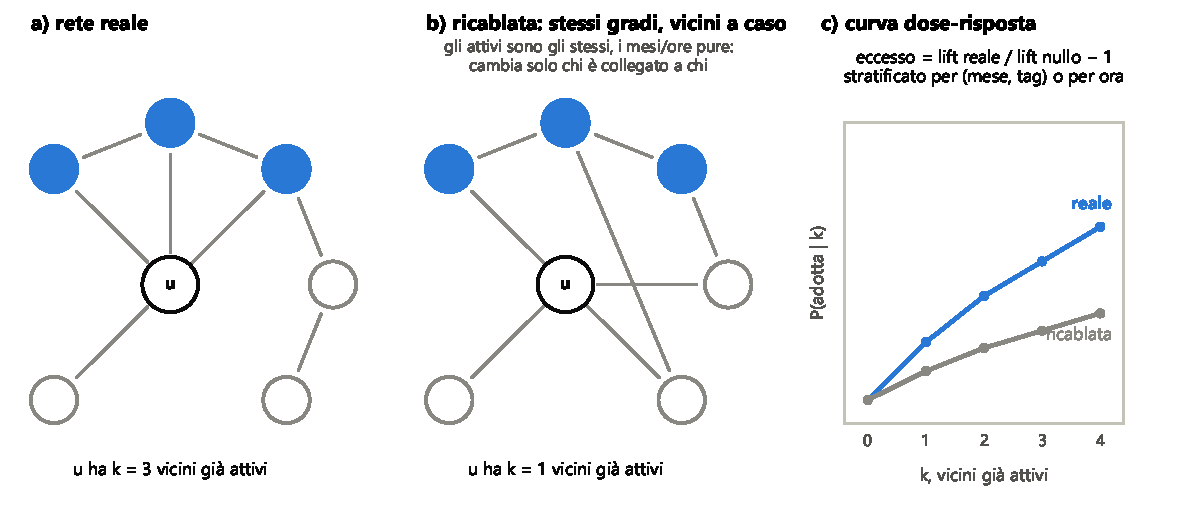
\includegraphics[width=\textwidth]{schema_dose}
  \caption{Il test dose-risposta. (a)~Nella rete reale $u$ ha $k$ vicini già attivi. (b)~Nella rete ricablata ogni nodo mantiene il proprio grado e i propri tempi, ma i vicini sono estratti a caso. (c)~Se la curva reale sale più di quella ricablata, la topologia specifica conta oltre grado e attività.}
  \label{fig:dose}
\end{figure}

\subsection{Fase 1: le comunità}
\label{sec:met-fase1}
\dovesiamo{Fase 1 della pipeline di ottimizzazione.}{i livelli della rete visibili prima del confine.}{una partizione dei nodi in comunità, che la Fase 3 userà per il vincolo di diversità e la previsione come attributi.}{$\Qtras$, fuori campione, sulle trasmissioni avvenute dopo il confine.}
Le comunità servono da \emph{barriere} nella Fase~3 e da \emph{attributi} nella previsione (\S\ref{sec:met-scala}): non descrivono di che cosa si parla, dicono lungo quali canali l'influenza passa. Il criterio con cui si sceglie la partizione deve rispecchiarlo, e deve essere fuori campione.

\paragraph{Le candidate.} Cinque partizioni, più un controllo:
\begin{itemize}
  \item \emph{F follower}: Leiden \citep{traag2019} sul solo grafo dei follower, simmetrizzato (la modularità è definita su grafi non orientati, e per le comunità conta che due utenti siano collegati, non in che verso), con la modularità come obiettivo;
  \item \emph{F Louvain}: lo stesso grafo con Louvain \citep{blondel2008}, per misurare quanto pesi qui la garanzia di comunità connesse che Leiden aggiunge;
  \item \emph{RT} e \emph{MT}: Leiden sui soli livelli di interazione, che lasciano isolati quasi tutti i nodi;
  \item \emph{fusione convenzionale}: Leiden sulla somma dei quattro livelli, ciascuno diviso per il proprio peso totale, la normalizzazione standard, che fa pesare un retweet quanto circa cinquecento archi di follow;
  \item \emph{fusione calibrata}: come sopra, ma con gli strati di interazione moltiplicati per un coefficiente $\lambda$ scelto dal dato (sotto);
  \item \emph{controllo}: ogni nodo nella propria comunità.
\end{itemize}
Il calcolo passa per igraph \citep{csardi2006} e leidenalg \citep{traag2019}: dodici milioni e mezzo di archi non sono per NetworkX, e la scelta è dettata dalla scala prima che dall'algoritmo.

\paragraph{Il criterio decisionale, $\Qtras$.} Il problema di ogni community detection è che l'algoritmo ottimizza una funzione (la modularità sulla rete che gli si dà) e, se lo si giudica con la stessa funzione sulla stessa rete, si valuta da solo. Serve un giudice che non abbia visto la rete su cui la partizione è stata calcolata, e che misuri ciò che le comunità devono servire a fare: dire lungo quali canali passa la diffusione. Il giudice è la \emph{rete di trasmissione realizzata}: l'insieme degli archi di follow $u \to v$ tali che $v$ ha adottato dopo il confine e $u$ era già attivo al momento dell'adozione di $v$, i canali lungo cui l'influenza \emph{può} essere davvero passata, 5.567.867 archi su 96 ore di verifica. La procedura, passo per passo:
\begin{enumerate}
  \item si calcola la partizione con i soli dati precedenti all'ora 72;
  \item si costruisce la rete di trasmissione con le adozioni \emph{successive} all'ora 72: per ogni utente $v$ che adotta all'ora $h > 72$, e per ogni $u$ che $v$ segue e che era già attivo prima di $h$, un arco $u \to v$;
  \item si calcola la modularità~(\ref{eq:modularita}) di quella rete rispetto alla partizione del passo 1: è $\Qtras$;
  \item si confrontano le candidate su $\Qtras$, con l'intervallo bootstrap della differenza (\S\ref{sec:protocollo}).
\end{enumerate}
$\Qtras$ alto vuol dire che le trasmissioni realizzate sono rimaste in gran parte \emph{dentro} le comunità, molto più di quanto ci si aspetterebbe da comunità delle stesse dimensioni disposte a caso. Due letture più semplici lo accompagnano nei risultati: la \emph{quota intra}, cioè la frazione di trasmissioni con i due estremi nella stessa comunità, e il suo rapporto con la quota che darebbe un'assegnazione casuale dei nodi a comunità delle stesse dimensioni (la somma dei quadrati delle frazioni di nodi per comunità). La modularità porta dentro di sé il modello nullo a gradi preservati, è per definizione \emph{intra osservato meno intra atteso}, e quindi non premia né la partizione unica né quella a singoletti. Ed è fuori campione per costruzione: la partizione si calcola su ciò che si vede prima dell'ora 72, e si giudica su ciò che succede dopo.

Come criterio di supporto si calcola l'\emph{AMI} \citep{vinh2010} fra la partizione e l'ora di adozione dei bersagli: le comunità si accendono insieme? È una verità completamente indipendente dalla topologia. Si calcola anche l'NMI, ma solo per mostrare in che misura inganna.

\paragraph{L'accoppiamento $\lambda$.} La rete di lavoro della fusione calibrata è
\begin{equation}
  A(\lambda) \;=\; \frac{A_F}{\|A_F\|} \;+\; \lambda \sum_{\ell \in \{\mathrm{RT},\mathrm{MT},\mathrm{RE}\}} \frac{A_\ell}{\|A_\ell\|},
\end{equation}
dove $\|A_\ell\|$ è il peso totale del livello $\ell$. Dividere ogni livello per il proprio peso totale è la \emph{normalizzazione convenzionale}, e con $\lambda = 1$ fa pesare ogni livello quanto gli altri: i 29.444 archi di retweet contano, in totale, quanto i 14,8 milioni di archi di follow, cioè ogni singolo retweet vale circa cinquecento archi di follow. È una scelta ragionevole quando i livelli hanno dimensioni confrontabili, ed è quella che di solito si adotta senza dirlo; qui i livelli differiscono di tre ordini di grandezza, e la scelta va messa alla prova. Il coefficiente $\lambda$ lo fa: $\lambda = 1$ è la convenzione, $\lambda = 0$ è il solo follower, e in mezzo gli strati di interazione entrano con un peso ridotto.

$\lambda$ si sceglie su una griglia $\{0, 0{,}003, 0{,}01, 0{,}03, 0{,}1, 0{,}3, 1\}$, e la procedura è la stessa di $\Qtras$ ma confinata al periodo di addestramento: per ogni valore della griglia si costruisce $A(\lambda)$, si calcola la partizione con Leiden, e la si giudica con la modularità sulle trasmissioni \emph{precedenti} al confine, gli archi $u \to v$ in cui $v$ ha ritwittato $u$ prima dell'ora 72. Si tiene il $\lambda$ che massimizza quella modularità. La finestra di verifica non entra nella scelta: è \emph{in campione} per la scelta di $\lambda$ e \emph{fuori campione} per il verdetto, che si dà solo dopo su $\Qtras$. Se il $\lambda$ scelto fosse zero, la conclusione «il multistrato non paga su questo substrato» sarebbe una misura e non una convenzione.

\subsection{Fase 2: le probabilità}
\label{sec:met-fase2}
\dovesiamo{Fase 2 della pipeline di ottimizzazione.}{il grafo dei follower e il log delle attività prima del confine.}{una probabilità di trasmissione $p(u,v)$ per ogni arco di follow, e la scala a cui usarla.}{l'errore di stima sugli archi di test, e il regime (sotto o sopra la soglia di percolazione).}
Per simulare una diffusione serve $p(u,v)$, la probabilità che $u$ attivi $v$. Non viene assegnata: viene stimata dal log, e poi estesa dove il log tace.

\paragraph{Credit distribution orientata.} Nella variante statica di Bernoulli di \citet{goyal2010},
\begin{equation}
  p(u \to v) \;=\; \frac{\mathrm{trasmissioni}(u \to v)}{\mathrm{attività}(u) + s},
  \label{eq:credit}
\end{equation}
dove le trasmissioni sono gli eventi precedenti al confine in cui $v$ ha ritwittato, menzionato o risposto a $u$, l'attività di $u$ è il numero di volte in cui $u$ compare nel log prima del confine, le occasioni in cui poteva influenzare chi lo segue, e $s = 5$ è uno smoothing che impedisce a un utente con una sola comparsa copiata una volta di ottenere $p = 1$. La stima è definita solo sugli archi di follow, e solo nel verso del follow: mettere un $p$ dove il canale non esiste gonfierebbe la diffusione con archi che nessuno può percorrere. Su \hg{} il numeratore è un evento \emph{osservato}: il retweet è la dichiarazione di aver copiato. Su \sx{} era una coincidenza temporale fra due adozioni, e la differenza si vede nei risultati. Gli archi con almeno una trasmissione, i \emph{ricchi}, sono 28.498, lo 0,19\% del totale.

\paragraph{GraphSAGE sugli archi.} Una rete a due strati di aggregazione \citep{hamilton2017} estende la stima ai 14,8 milioni di archi \emph{poveri}. Gli attributi dei nodi sono 42: grado entrante e uscente su ciascuno dei quattro livelli, l'indicatore di attività pre-confine e l'ora della prima comparsa, e trentadue dimensioni spettrali del grafo dei follower (SVD troncata randomizzata \citep{halko2011} dell'adiacenza simmetrizzata), che portano la posizione del nodo nella struttura globale. I due strati producono per ogni nodo una rappresentazione $h$ (32 numeri) che riassume i suoi attributi e quelli del vicinato a distanza due. La testa, un piccolo MLP, prende la coppia $(h_u, h_v)$ dell'arco, ne forma prodotto, somma e differenza assoluta, vi aggiunge gli attributi dell'arco (il logaritmo delle attività dei due estremi, cioè il denominatore della~(\ref{eq:credit}), che la rete deve poter vedere) e produce $p(u,v)$ attraverso una sigmoide. L'addestramento minimizza l'errore quadratico fra questa $p$ e quella della credit distribution sugli archi ricchi. Tre scelte contano:
\begin{itemize}
  \item si addestra su un solo verso per arco: aggiungere il verso opposto con bersaglio zero insegnerebbe «assenza di canale» come se fosse «influenza nulla»;
  \item si campionano quattro archi \emph{negativi} (follow senza trasmissione, bersaglio zero) per ogni arco ricco, altrimenti la rete vede un mondo in cui la trasmissione è la norma e sovrastima sui poveri;
  \item il bias d'uscita parte dal logit della media dei bersagli: senza, l'epoca zero prevede 0,5 contro bersagli che valgono in media 0,01, e l'ottimizzatore non arriva nemmeno alla costante ottima nel numero di epoche disponibili.
\end{itemize}
Gli archi campionati si dividono 70/15/15; l'arresto anticipato guarda il 15\% di validazione, l'MSE riportato viene dal 15\% di test. Il primo prodotto sparso $A x$ è costante durante l'addestramento e si calcola una volta sola: è una riscrittura esatta che dimezza il costo per epoca. La variante con la perdita pesata sul grado del nodo di arrivo (l'ipotesi che l'MSE uniforme trascuri gli hub, che sono ciò che il greedy guarda) viene addestrata e messa alla prova allo stesso modo.

\paragraph{Taratura del regime.} Sotto Independent Cascade la diffusione ha una soglia di percolazione (\S\ref{sec:background}): ciò che percola è l'attivazione, lungo il sottografo degli archi «vivi», e sopra soglia una cascata partita da un nodo qualunque raggiunge una componente gigante. Sopra soglia succede una cosa che rovina in silenzio ogni confronto a valle: gli insiemi RR diventano enormi, migliaia di nodi hanno copertura marginale equivalente, e il greedy sceglie fra pari in modo arbitrario. Il controllo è guardare la dimensione media degli insiemi RR al variare di un fattore di scala su $p$, e scegliere il fattore più grande che la tiene fra 3 e 30 nodi. Due dettagli non ovvi: la taratura va fatta sulla matrice \emph{che si userà davvero} (la $p$ della GNN, non la mediana costante sugli archi poveri), perché alla stessa scala i due sistemi differiscono di un ordine di grandezza (25,7 contro 1,59 nodi per insieme), e la griglia si percorre in salita fermandosi al primo punto sopracritico, dove un solo insieme RR può toccare centomila nodi.

\paragraph{Non stazionarietà.} Per ogni ora $h$ si contano gli archi di follow \emph{a rischio} ($u$ già adottante, $v$ non ancora) e quanti di questi trasmettono, cioè $v$ adotta in $h$. Il rapporto è il tasso di trasmissione per arco-ora; il rapporto fra la sua media dopo il confine e prima è il \emph{fattore di non stazionarietà}. È la stessa quantità che la taratura chiama scala, ma stimata dal dato invece che scelta per portare gli insiemi RR in un intervallo comodo.

\subsection{Fase 3: i seed}
\label{sec:met-fase3}
\dovesiamo{Fase 3, l'ultima della pipeline di ottimizzazione.}{la $p$ della Fase 2 e la partizione della Fase 1.}{un insieme di $k$ seed per ogni budget $k$ e ogni peso $\alpha$ del vincolo di diversità.}{qui la diffusione simulata dentro il modello; il giudizio esterno viene dopo, nella validazione.}
\paragraph{TIM con RR-sketch.} Si generano 120.000 insiemi RR \citep{borgs2014,tang2014} con la $p$ della Fase~2 alla scala tarata, e il greedy sceglie $k$ seed per massima copertura (figura~\ref{fig:rr}). Gli insiemi si generano una volta e si tengono in cache, con la scala nel nome del file, perché un campionamento fatto per un regime e riletto dopo che il regime è cambiato sarebbe un errore silenzioso.

\paragraph{Il vincolo di diversità.} È il criterio~(\ref{eq:dtim}), spiegato termine per termine in \S\ref{sec:bg-dtim}, con una soglia: il premio vale solo per comunità con almeno 200 nodi (lo 0,04\% della rete, la stessa frazione che 50 nodi erano su \sx{}). Senza la soglia, su \sx{} il vincolo spendeva seed per aprire comunità da due nodi, e il numero di comunità raggiunte cresceva senza che crescesse nulla di sostanziale. Si misura la \emph{superficie} $k \times \alpha$: per $k \in \{5,10,20,50\}$ e $\alpha \in \{1, 0{,}95, 0{,}9, 0{,}8, 0{,}7, 0{,}5, 0{,}3\}$, quante comunità toccano i seed e quanto costa in diffusione attesa, stimata Monte Carlo con 1.200 simulazioni. Il rumore Monte Carlo di una singola stima si misura ripetendola con sei semi diversi, e si riporta accanto alla superficie: sotto quel rumore le celle non si distinguono.

\paragraph{L'ablazione della GNN, a regime pareggiato.} La domanda è se la $p$ appresa produca seed diversi da una $p$ costante. Alla scala nominale le due finirebbero in regimi separati da due ordini di grandezza (2.400 nodi per insieme RR contro 29) e il confronto misurerebbe il regime, non il modello. Ogni variante viene quindi portata per bisezione alla stessa dimensione media degli insiemi RR, e solo allora si confrontano i seed: per sovrapposizione degli insiemi di seed (quanti seed su $k$ sono in comune: «23/50» vuol dire 23 seed uguali su 50), per correlazione di Spearman \citep{spearman1904} delle coperture, e per diffusione attesa sotto ciascun modello. Il metro è il \emph{pavimento di rumore}: lo stesso modello con un altro seme casuale. Se ne riportano due, il massimo fra le auto-consistenze (permissivo) e il minimo (severo), e si giudica sul secondo.

\subsection{Chi adotterà: la scala a pioli}
\label{sec:met-scala}
\dovesiamo{fuori dalla pipeline di ottimizzazione, si fa previsione.}{per ogni utente non ancora attivo, attributi calcolati con i soli dati precedenti al confine.}{una probabilità $\phat(v)$ che l'utente adotti dopo, che diventerà il peso dell'IM pesata.}{l'AUC su utenti di test mai visti.}
La validazione (\S\ref{sec:ris-validazione}) mostra che l'ottimizzatore non sa chi adotterà. Questa parte glielo insegna, e nel farlo misura quale informazione conta.

\paragraph{Il problema, in parole.} Ci si mette all'ora 72. Ci sono 421.017 utenti che non hanno ancora detto nulla dell'Higgs. Di questi, nei quattro giorni successivi, 269.081 ne parleranno e 151.936 no. La domanda è: guardando solo ciò che si vede \emph{adesso} (quanti seguaci ha un utente, quanti dei suoi seguiti stanno già parlando dell'evento, com'è fatta la sua comunità, dove sta nella rete) si riesce a dire chi dei due gruppi sarà? È una classificazione binaria sui nodi. Non si chiede \emph{quando} adotterà, né \emph{da chi} lo verrà a sapere: solo se.

Il modo in cui la si affronta serve a due cose insieme. La prima è produrre una $\phat(v)$ utilizzabile dall'ottimizzatore (\S\ref{sec:met-im-pesata}). La seconda, più importante, è \emph{misurare quale informazione strutturale predice l'adozione}: e per questo il classificatore non si costruisce in un colpo solo, ma per gradini. Ogni gradino aggiunge una famiglia di attributi al precedente e riaddestra lo stesso modello; la differenza di accuratezza fra un gradino e il precedente è la misura di quanto quella famiglia porta, \emph{al netto} di tutto ciò che c'era già. Se le comunità aggiungono molto sopra l'esposizione, non è perché «sono correlate con l'adozione» (lo è quasi tutto) ma perché dicono qualcosa che grado ed esposizione non dicevano.

\paragraph{Come si legge l'AUC.} L'\emph{area sotto la curva ROC} \citep{fawcett2006} è la probabilità che, presi a caso un utente che ha adottato e uno che non ha adottato, il modello dia al primo un punteggio più alto del secondo. Vale 0,5 per un modello che tira a caso e 1 per uno perfetto. Non dipende da una soglia di decisione, e non è sensibile allo sbilanciamento delle classi (qui il 64\% adotta): per questo è la metrica primaria. Un'AUC di 0,68 vuol dire che in due casi su tre il modello ordina correttamente una coppia adottante/non adottante: utile, non impressionante.

\paragraph{Popolazione ed etichetta.} La popolazione sono i 421.017 utenti non attivi all'ora 72; l'etichetta è 1 se adottano entro l'ora 168 (269.081, il 63,9\%), 0 altrimenti. La divisione è 70/15/15 sui nodi, stratificata sull'etichetta, con seme fisso: il 15\% di validazione serve solo all'arresto anticipato dei modelli neurali, il 15\% di test non viene guardato prima della fine.

\paragraph{Le famiglie di attributi.} Tutti calcolabili prima dell'ora 72; la verità di riferimento è la sola cosa che vive dopo, e la si tocca in un posto solo. In ordine di impilamento, con accanto la domanda a cui ciascuna famiglia risponde:
\begin{enumerate}
  \item \emph{grado} (2 attributi): seguaci e seguiti, in logaritmo. \emph{Quanto sei grande?} È il punto di partenza obbligato, perché è l'informazione che il cancello ha già isolato come «non topologia»: tutto ciò che viene dopo va misurato al netto di questo;
  \item \emph{esposizione} (4): quanti dei miei seguiti erano già attivi al confine, in conteggio e in quota; quanti dei miei seguaci (omofilia osservabile, non canale, perché i loro tweet non mi raggiungono); l'ora della prima esposizione. \emph{Quanto dell'evento ti sta già arrivando?} È la dose della curva dose-risposta, resa attributo;
  \item \emph{comunità} (4): la dimensione della mia comunità nella partizione scelta dalla Fase~1, la quota di essa già accesa, quanta della mia esposizione viene da dentro, in conteggio e in quota. \emph{Il tuo gruppo si sta accendendo?} Le comunità entrano come \emph{numeri}, non come identità categorica: un attributo che vale solo dentro la propria comunità non generalizza, e comunque la domanda è se \emph{essere in una comunità che si sta accendendo} predice l'adozione, non se la comunità 17 adotta più della 23;
  \item \emph{spettro} (32): le trentadue dimensioni spettrali del grafo dei follower, la posizione del nodo nella struttura globale. \emph{In quale regione della rete stai?} È ciò che né il grado né i vicini a un passo dicono;
  \item \emph{propagati} (126): gli attributi precedenti mediati sui vicini e sui vicini dei vicini, $[x,\, \tilde{A}x,\, \tilde{A}^2 x]$ con $\tilde{A}$ l'adiacenza simmetrizzata normalizzata per riga. \emph{Com'è fatto il tuo vicinato, in media?} È la stessa aggregazione che fa una GNN, ma calcolata una volta e data a un modello ad alberi: serve a separare, nel gradino successivo, il contributo dell'aggregazione da quello della rete neurale.
\end{enumerate}
Un esempio, ipotetico ma tipico, aiuta a vedere che cosa il modello guarda. Un utente con 300 seguiti, di cui 40 già attivi all'ora 72 (quota 0,13), la cui comunità ha 20.000 membri di cui il 9\% già attivo, e per cui 35 dei 40 seguiti attivi stanno nella sua stessa comunità (quota intra 0,88): esposto, dentro un gruppo che si sta accendendo, e con un'esposizione che viene da dentro. È il profilo a cui la scala assegna $\phat$ alta. Un utente con 3.000 seguiti di cui 5 attivi, in una comunità grande e fredda, ha un grado più alto ma una $\phat$ più bassa: ed è il caso in cui l'esposizione batte il grado.

\paragraph{I modelli.} Il modello è addestrato sul 70\% dei nodi: vede i loro attributi e la loro etichetta (adotta / non adotta), e impara una funzione dagli attributi alla probabilità. Poi la si applica ai nodi di test, di cui l'etichetta non è mai stata letta, e si misura l'AUC. I primi cinque gradini usano lo stesso modello, il gradient boosting a istogrammi di scikit-learn \citep{pedregosa2011}, nello stile di LightGBM \citep{ke2017}, a iperparametri fissi (300 iterazioni al massimo, 31 foglie, passo 0,08, arresto anticipato su un decimo dell'addestramento): non c'è ricerca, perché la domanda è quale famiglia porta informazione, e una ricerca per gradino confonderebbe «attributi migliori» con «modello tarato meglio». Il sesto gradino è la GNN, \textbf{SIGN} \citep{frasca2020}: gli stessi attributi propagati del quinto, dati a un MLP (128--64--1, dropout 0,2, Adam a $10^{-3}$, mini-batch da 8.192, arresto anticipato sull'AUC di validazione). La differenza fra il quinto e il sesto gradino isola il solo effetto della non-linearità sull'aggregazione, a parità di ingresso.

La scelta di SIGN al posto di una GraphSAGE a nodi end-to-end è imposta dalla scala: a batch pieno su 456.627 nodi la GraphSAGE impiegava 95 secondi a epoca e dopo 200 epoche, 5,3 ore, non era ancora convergita (AUC di validazione 0,6666). Precalcolare la propagazione e addestrare sopra fa lo stesso lavoro in 92 secondi, e arriva più in alto.

\paragraph{Il settimo gradino: R-SIGN.} SIGN propaga sull'adiacenza simmetrizzata del solo follower: fonde seguiti e seguaci e non vede gli strati di interazione. R-SIGN tiene separate direzione e tipo di relazione con dieci operatori (figura~\ref{fig:schema-rsign}): $x$; $A_{\mathrm{in}} x$ e $A_{\mathrm{out}} x$ (media sui seguiti e sui seguaci); le quattro combinazioni a due passi; e $A_{\mathrm{in}} A_{\ell}\, x$ per $\ell \in \{\mathrm{RT},\mathrm{MT},\mathrm{RE}\}$: con chi i miei seguiti hanno ritwittato, menzionato, risposto. Ogni blocco ha una propria matrice di pesi $W_r$ (da 42 a 32 dimensioni), le proiezioni si concatenano e passano per lo stesso MLP. È il primo strato di un R-GCN \citep{schlichtkrull2018} senza la non-linearità fra le aggregazioni: un R-GCN vero, a batch pieno su questa scala, non è praticabile su CPU, e la differenza è dichiarata. Lo si confronta in due modi: gli attributi relazionali dati agli stessi alberi (isola l'informazione, a parità di modello) e R-SIGN contro SIGN (la GNN).

\paragraph{Valutazione.} AUC \citep{fawcett2006} come metrica primaria, average precision come secondaria, sul test. L'incertezza viene da un bootstrap appaiato a grappoli \emph{sulle comunità} (\S\ref{sec:protocollo}), con Bonferroni sui confronti fra gradini consecutivi. Il rumore di riferimento per l'ultimo gradino è la GNN rieseguita con un altro seme: se la differenza fra due modelli non supera quella fra due semi dello stesso modello, non è un effetto.

\begin{figure}[htbp]
  \centering
  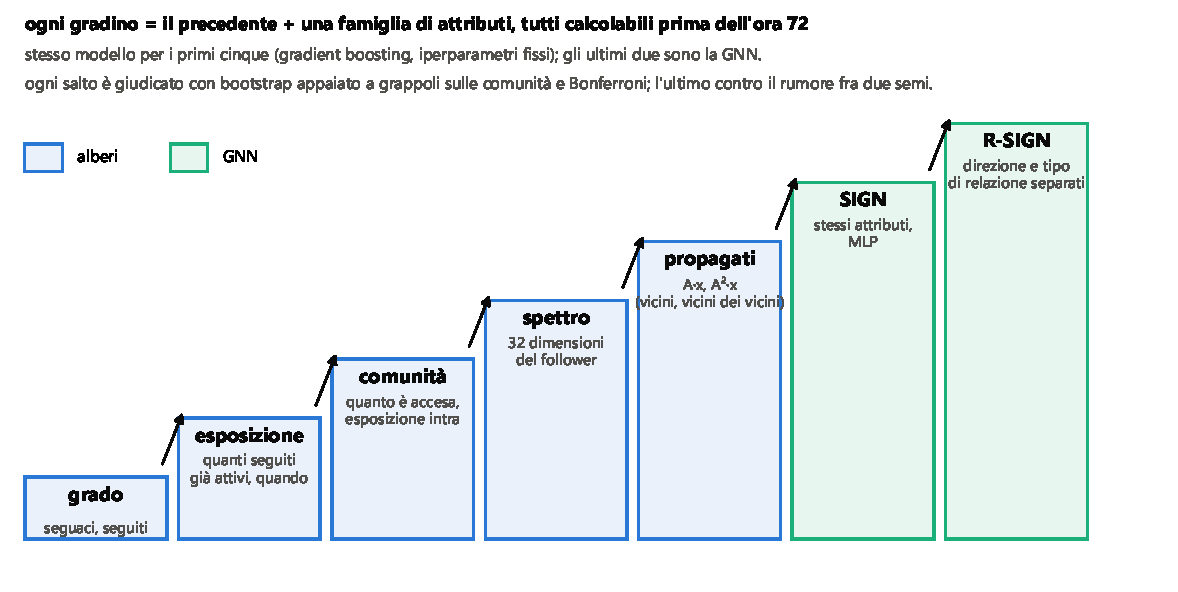
\includegraphics[width=\textwidth]{schema_scala}
  \caption{La scala a pioli. Ogni gradino è il precedente più una famiglia di attributi; il modello è lo stesso per i primi cinque, gli ultimi due sono la GNN. La differenza fra un gradino e il precedente misura l'informazione che quella famiglia porta.}
  \label{fig:schema-scala}
\end{figure}

\begin{figure}[htbp]
  \centering
  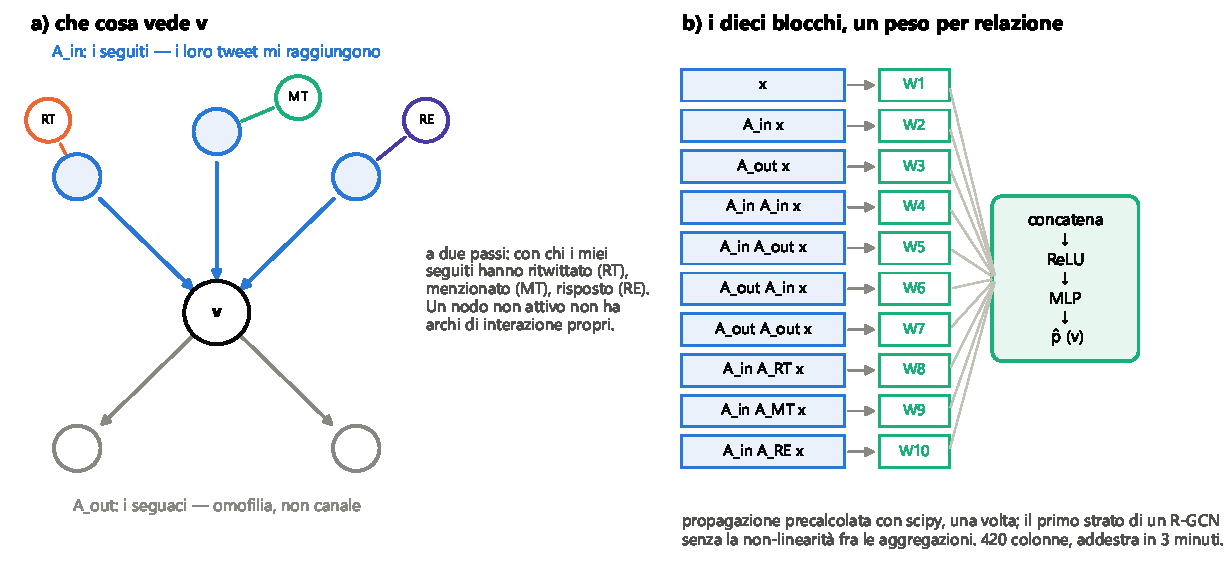
\includegraphics[width=\textwidth]{schema_rsign}
  \caption{R-SIGN. (a)~Ciò che il nodo $v$ vede: i seguiti (il canale), i seguaci (omofilia osservabile), e a due passi con chi i seguiti hanno ritwittato, menzionato, risposto — un nodo non attivo non ha archi di interazione propri. (b)~I dieci operatori di propagazione, un blocco di pesi ciascuno, poi un MLP: il primo strato di un R-GCN senza la non-linearità fra le aggregazioni.}
  \label{fig:schema-rsign}
\end{figure}

\subsection{IM pesata dalla previsione}
\label{sec:met-im-pesata}
\dovesiamo{previsione e ottimizzazione insieme.}{la $p$ della Fase 2 e la $\phat$ della scala.}{seed.}{la stessa validazione esterna, nel confronto diretto col grado.}
TIM+ massimizza il numero atteso di nodi attivati, e per questo perde contro il grado (\S\ref{sec:ris-validazione}): non tutti i nodi valgono uguale, e non sa quali. Il classificatore della scala lo sa un po'. L'ultimo capitolo li mette insieme.

\paragraph{Radici pesate.} Nel campionamento a raggiungibilità inversa la radice di ogni insieme RR è uniforme sui nodi, e la copertura stima il \emph{numero} di nodi attivati. Se la radice si estrae in proporzione a un peso $w(v)$, la copertura stima la \emph{somma dei pesi} dei nodi attivati \citep{borgs2014}. Con $w(v) = \phat(v)$, la probabilità prevista che $v$ adotti, il greedy massimizza gli adottanti probabili. Ai 35.610 utenti già attivi si dà peso zero: non sono bersagli.

\paragraph{Fuga di informazione, e come si evita.} Il classificatore ha visto le etichette dei nodi di addestramento. Se le sue probabilità pesassero le radici, i seed sarebbero scelti da un modello che conosce parte della verità su cui poi vengono giudicati. Le probabilità si producono quindi \emph{out-of-fold}: cinque fold stratificati, ogni nodo pesato da un modello (gradient boosting sugli attributi propagati) che non ha mai visto la sua etichetta. L'AUC out-of-fold, 0,6731, è praticamente quella del gradino corrispondente.

\paragraph{Confronti.} Quattro strategie a parità di budget (TIM+ non pesato, TIM pesato, TIM pesato con il vincolo di diversità a $\alpha = 0{,}80$, e il grado uscente), sul criterio esterno della validazione, per $k \in \{10, 20, 50\}$. Il confronto che conta è quello diretto col grado, e viene riportato come tale. Un controllo in più: gli stessi seed, valutati alla trasmissività misurata del periodo di verifica ($\times 4{,}55$), sopra la soglia di percolazione. \emph{Scegliere} sopra soglia non ha senso, perché migliaia di nodi sono equivalenti; \emph{valutare} un insieme già fissato si può, e se la graduatoria regge nei due regimi non è un artefatto della taratura.

% =====================================================================
\clearpage
\section{Protocollo sperimentale}
\label{sec:protocollo}

Il protocollo è la parte del lavoro che decide che cosa conta come risultato, e per questo viene prima dei risultati. Le sue regole sono tre (il criterio è esterno, l'incertezza è appaiata e a grappoli, la fuga di informazione è chiusa per costruzione) e valgono per ogni esperimento della relazione.

\subsection{Il criterio esterno}
Tutte le misure delle tre fasi vivono \emph{dentro} il modello: la diffusione attesa di un insieme di seed è una simulazione di Independent Cascade con la stessa $p$ che ha scelto i seed, e un confronto fatto lì dentro può solo confermare le proprie premesse. Ogni modello preferisce i propri seed, e la sezione~\ref{sec:ris-validazione} lo mostra alla lettera.

Il criterio che decide è quindi esterno. Per una strategia di seed $S$, scelta con soli dati precedenti al confine, si stima Monte Carlo la probabilità $\pi_S(v)$ che ciascun nodo venga attivato partendo da $S$ (3.000 simulazioni per la validazione, 2.000 per l'IM pesata), e il punteggio è
\begin{equation}
  \mathrm{punteggio}(S) \;=\; \sum_{v \in \mathcal{B}} \pi_S(v),
\end{equation}
dove $\mathcal{B}$ sono i 269.081 utenti che hanno \emph{davvero} adottato dopo il confine. Un modello che mette probabilità alta su chi ha effettivamente adottato prende molto; uno che la mette altrove prende poco. Nessuna simulazione decide chi ha ragione: lo decide il log. La stessa logica vale per la classificazione dell'adozione, dove il criterio è l'AUC sui nodi di test, la cui etichetta non è mai stata vista.

Il criterio ha un limite che va detto: $\pi$ è pur sempre calcolata con la $p$ del modello, quindi il punteggio misura quanto il modello \emph{indirizza} verso i veri adottanti, non quanto la cascata reale sia riprodotta. È per questo che si riporta anche il potere esplicativo assoluto (\S\ref{sec:ris-validazione}), che è piccolo, e che i confronti sono sempre relativi e appaiati.

\subsection{Bootstrap appaiato a grappoli}
L'incertezza di ogni confronto viene da un bootstrap con due proprietà, entrambe necessarie \citep{efron1994}.

\paragraph{Appaiato.} La stessa replica alimenta tutte le strategie, e si prendono i percentili della \emph{differenza}. Se una replica pesca ore, tag o comunità in cui la diffusione è grande, tutte le strategie ne beneficiano, e nella differenza la variabilità comune si cancella. Senza l'appaiamento gli intervalli sarebbero dominati dalla variabilità fra unità, che non è ciò che si vuole misurare. Il $p$-value è la frazione di repliche in cui la differenza cambia segno rispetto a quella osservata, raddoppiata perché il test è a due code: $p = 0{,}19$ vuol dire che in circa una replica su dieci il perdente diventa vincitore. Un $p$ piccolo dice che l'ordine fra le due strategie è stabile sotto ricampionamento; un $p$ grande che è casuale. L'intervallo dice lo stesso in un'altra forma: se contiene lo zero, non c'è un vincitore.

\paragraph{A grappoli.} L'unità di ricampionamento non è la singola osservazione ma il gruppo di osservazioni dipendenti, e cambia da esperimento a esperimento perché cambia la struttura di dipendenza (tabella~\ref{tab:protocollo}). Su \sx{} è il \emph{tag}: le esposizioni dello stesso tag appartengono alla stessa cascata, e trattarle come indipendenti stringe gli intervalli di circa tre volte. Su \hg{}, per tutto ciò che si somma sul tempo ($\Qtras$, la validazione dei seed, l'IM pesata) è l'\emph{ora} di adozione: le trasmissioni della stessa ora sono la stessa ondata. Per la classificazione dell'adozione è la \emph{comunità}: i nodi della stessa comunità si assomigliano per costruzione (stessa quota di attivi, stessa regione dello spettro), e sono l'unità di dipendenza più larga disponibile.

Il ricampionamento è per pesi. Estrarre i grappoli con reinserimento equivale a dare a ogni osservazione un peso pari a quante volte il suo grappolo è stato estratto; quando la statistica è una somma sui grappoli, come $\Qtras$ o il punteggio di validazione, una replica costa un prodotto matrice-vettore invece di una ricostruzione, e quando è un'AUC si usa il peso come peso di campione. Duemila repliche ovunque, tremila per la validazione.

\paragraph{Bonferroni, e il rumore di riferimento.} Mettendo alla prova più candidati contro lo stesso riferimento, la probabilità che almeno uno risulti diverso per caso cresce col numero di confronti; la correzione di Bonferroni \citep{dunn1961} divide la soglia per il numero di confronti: quella riportata in tabella~\ref{tab:protocollo} è $0{,}05/m$ con $m$ confronti, e un risultato che passa lo 0,05 ma non la soglia corretta è riportato come «al limite», non come vittoria. Dove il confronto è fra due modelli addestrati, c'è un secondo metro: lo stesso modello rieseguito con un altro seme casuale. Se la differenza fra due modelli non supera quella fra due semi dello stesso modello, non è un effetto, qualunque sia il $p$. Per le stime Monte Carlo il rumore si misura allo stesso modo, ripetendo la stima con semi diversi, e si riporta accanto ai numeri che ne dipendono.

\begin{table}[htbp]
  \centering\small
  \caption{Per ogni esperimento, l'unità del bootstrap, il numero di confronti e la soglia corretta di Bonferroni.}
  \label{tab:protocollo}
  \footnotesize\setlength{\tabcolsep}{4pt}
  \begin{tabular}{llccl}
    \toprule
    esperimento & unità di ricampionamento & confronti & soglia & rumore di riferimento \\
    \midrule
    Fase 1, $\Qtras$ & l'ora di adozione (96) & 6 & 0,0083 & — \\
    Fase 3, superficie $k\times\alpha$ & — (Monte Carlo) & — & — & dev.\ st.\ fra semi MC: 0,12\% \\
    Validazione dei seed & l'ora di adozione (96) & 10 & 0,0050 & — \\
    Scala a pioli & la comunità (264) & 5 & 0,0100 & SIGN vs SIGN, altro seme \\
    Settimo gradino (R-SIGN) & la comunità (264) & 2 & 0,0250 & R-SIGN vs R-SIGN, altro seme \\
    IM pesata & l'ora di adozione (96) & 3 & 0,0167 & — \\
    \bottomrule
  \end{tabular}
\end{table}

\subsection{Fuga di informazione}
La fuga di informazione, cioè usare anche indirettamente ciò che si deve prevedere, è l'errore più facile da fare e il più difficile da vedere, perché produce risultati buoni. Il protocollo la chiude in quattro punti.

\begin{itemize}
  \item \emph{Il confine temporale.} Ogni attributo, partizione e stima usa solo eventi precedenti al confine; l'unica funzione che legge dopo è quella che produce l'etichetta, e sta da sola (\S\ref{sec:sistema}). Su \sx{}, dove il confine non bastava perché i tag bersaglio comparivano in più ruoli, si aggiunge la maschera severa: i bersagli sono esclusi anche dalla rete e dalla stima di $p$, non solo dalla verità di riferimento.
  \item \emph{Tre insiemi, non due.} Dove un modello ha un arresto anticipato, la decisione di quando fermarsi è una scelta di modello; farla guardando lo stesso insieme su cui poi si riporta la metrica significherebbe riportare un numero già ottimizzato. La divisione è 70/15/15: il 15\% di validazione decide l'arresto, il 15\% di test non viene mai letto prima della fine.
  \item \emph{Probabilità out-of-fold.} Il classificatore dell'adozione ha visto le etichette dei nodi di addestramento. Nell'IM pesata le sue probabilità pesano le radici degli insiemi RR, e i seed che ne escono vengono giudicati sulle stesse etichette: si producono quindi out-of-fold su cinque fold, in modo che nessun nodo sia pesato da un modello che ha visto la sua etichetta.
  \item \emph{La cache.} Un artefatto calcolato per una configurazione e riletto in un'altra è una fuga di informazione dal passato del progetto verso il presente. La scala di $p$ è parte del nome dei file degli insiemi RR, e le partizioni portano nel nome il livello e, per la fusione, il coefficiente.
\end{itemize}


% =====================================================================
\clearpage
\section{Risultati}
\label{sec:risultati}

\subsection{Il cancello}
\label{sec:ris-cancello}
\begin{figure}[htbp]
  \centering
  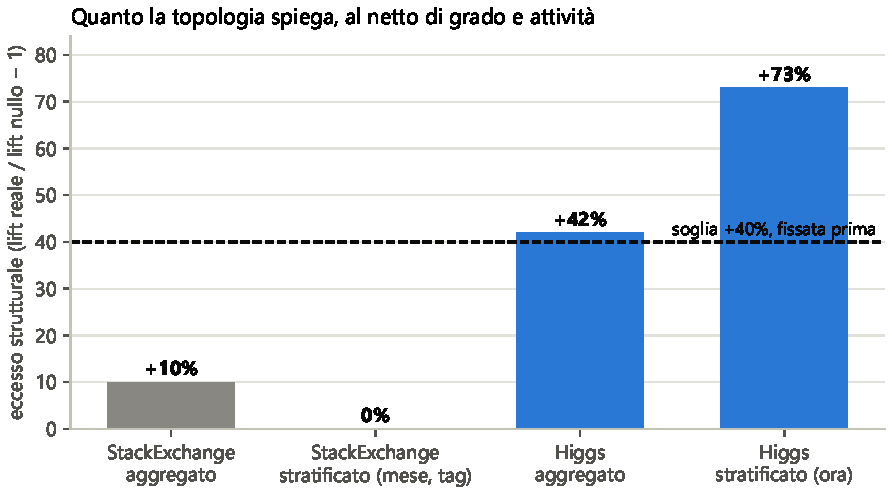
\includegraphics[width=0.8\textwidth]{fig_eccesso}
  \caption{L'eccesso strutturale sui due substrati. Su \sx{} il $+10\%$ aggregato sparisce stratificando per (mese, tag): era composizione del campione. Su \hg{} la stratificazione per ora lo porta a $+73\%$.}
  \label{fig:eccesso}
\end{figure}
Il cancello è stato misurato prima su \sx{}, dove il progetto era nato, e il risultato aggregato ($+10\%$, lift reale 2,19$\times$ contro 2,00$\times$ delle reti ricablate) sembrava poco ma non nullo. Stratificando per (mese, tag) l'eccesso \textbf{sparisce}: 1,54$\times$ reale contro 1,54$\times$ nullo, $-0\%$. Quel dieci per cento era interamente composizione del campione, cioè il fatto che nei mesi in cui un tag esplode quasi tutti sono esposti e quasi tutti adottano. La rete di risposte e commenti \emph{non porta} l'adozione dei tag: porta il grado e la popolarità, e basta.

Questo è anche la diagnosi retrospettiva della prima versione del progetto, che su \sx{} aveva prodotto un'ablazione della GNN nulla (1 seed su 50 contro un pavimento di rumore di 2), un vincolo di diversità a costo zero ma senza guadagno, e un esperimento competitivo dentro il rumore (appendice~\ref{app:stackexchange}). Non erano difetti di implementazione: si cercava struttura in un substrato che non ne ha.

Su \hg{} il primo tentativo, con la rete di retweet come substrato, è risultato degenere (\S\ref{sec:dati}). Con il grafo dei follower l'eccesso aggregato è $+42\%$ (lift 9,71$\times$ contro 6,82$\times$), appena sopra la soglia dei $+40\%$, e la stratificazione per ora lo porta a $\mathbf{+73\%}$: 3,39$\times$ contro 1,96$\times$. Qui la stratificazione lavora nel verso opposto rispetto a \sx{}: toglie l'effetto dell'ora di picco, che gonfiava il \emph{nullo} più del reale, e l'eccesso cresce. La topologia specifica del grafo dei follower spiega la maggior parte dell'esposizione. Le tre repliche del nullo differiscono fra loro di meno dell'1\% (deviazione standard del lift 0,05 su 6,82): l'incertezza del ricablaggio non è il problema.

La regola fissata prima ha dato il suo verdetto in entrambe le direzioni (no a \sx{}, sì a \hg{}) ed è questo che la rende una misura e non una giustificazione a posteriori. \sx{} resta nel lavoro come controllo negativo.

\subsection{Fase 1: quale partizione}
\begin{figure}[htbp]
  \centering
  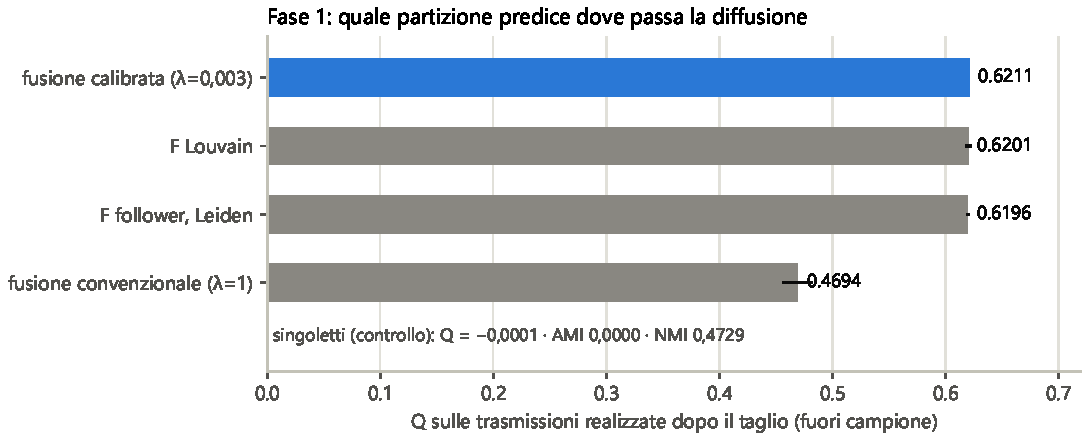
\includegraphics[width=0.85\textwidth]{fig_fase1_q}
  \caption{$\Qtras$ per partizione, con l'intervallo bootstrap della differenza dal riferimento. La fusione calibrata vince di poco ma con $p<0{,}001$; la fusione convenzionale perde il 24\%.}
  \label{fig:fase1}
\end{figure}
\begin{figure}[htbp]
  \centering
  \begin{subfigure}[t]{0.46\textwidth}
    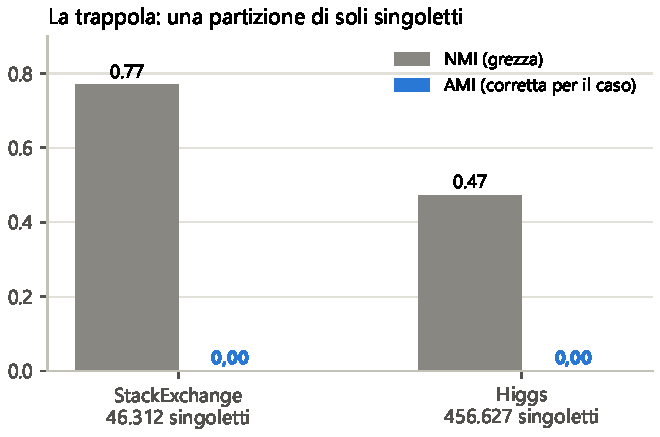
\includegraphics[width=\textwidth]{fig_nmi_ami}
    \caption{La trappola dell'NMI.}
    \label{fig:nmi}
  \end{subfigure}\hfill
  \begin{subfigure}[t]{0.52\textwidth}
    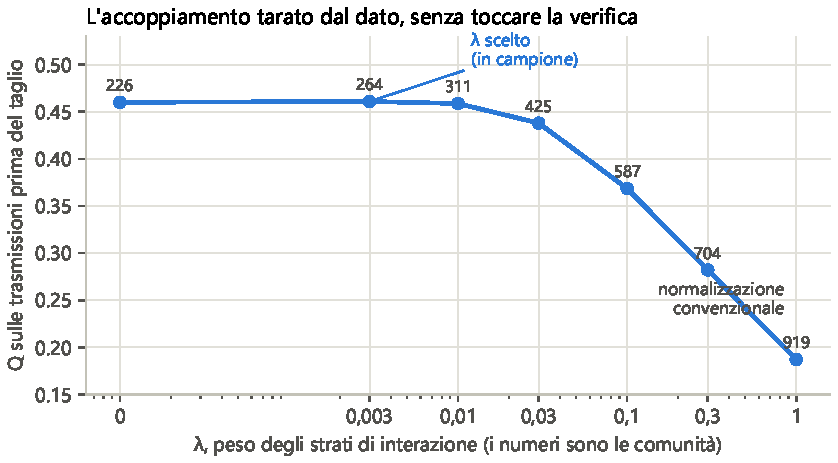
\includegraphics[width=\textwidth]{fig_accoppiamento}
    \caption{L'accoppiamento $\lambda$, scelto in campione.}
    \label{fig:accoppiamento}
  \end{subfigure}
  \caption{(a)~Una partizione di soli singoletti prende NMI 0,77 e 0,47 sui due substrati, e AMI zero. (b)~Il peso degli strati di interazione massimizza la modularità sulle trasmissioni precedenti al taglio a $\lambda=0{,}003$; a $\lambda=1$ (normalizzazione convenzionale) la partizione si frammenta in 919 comunità.}
\end{figure}

\begin{table}[htbp]
  \centering\small
  \caption{Fase 1 su \hg{}. Bootstrap appaiato a grappoli sull'ora, 2.000 repliche, riferimento la fusione calibrata.}
  \label{tab:fase1}
  \begin{tabular}{lrrrrl}
    \toprule
    partizione & com. & $\Qtras$ & AMI ora & NMI ora & vs riferimento \\
    \midrule
    fusione calibrata ($\lambda=0{,}003$) & 264 & \textbf{0,6211} & 0,0474 & 0,0497 & riferimento \\
    F Louvain & 321 & 0,6201 & 0,0498 & 0,0528 & $p=0{,}194$, equivalente \\
    F follower, Leiden & 226 & 0,6196 & 0,0476 & 0,0499 & $-0{,}0015$, $p<0{,}001$ \\
    fusione convenzionale ($\lambda=1$) & 919 & 0,4694 & 0,0380 & 0,0432 & $-0{,}1517$, $p<0{,}001$ \\
    controllo: singoletti & 456.627 & $-0{,}0001$ & 0,0000 & 0,4729 & $-0{,}6212$, $p<0{,}001$ \\
    \bottomrule
  \end{tabular}
\end{table}
\paragraph{Le comunità predicono dove passa la diffusione.} La partizione di lavoro, calcolata su ciò che si vede prima dell'ora 72, ha modularità $\Qtras = 0{,}6211$ sulla rete delle trasmissioni realizzate \emph{dopo}: il 74\% delle 5,57 milioni di trasmissioni resta dentro la comunità dell'influenzatore (la quota intra), contro il 10\% circa che darebbe un'assegnazione casuale dei nodi a comunità delle stesse dimensioni: 7,1 volte tanto. I due numeri sono la lettura semplice di $\Qtras$; la modularità li corregge anche per i gradi, ed è il criterio che decide. Su \sx{} lo stesso criterio dava 0,1274, e il criterio copriva il 10\% dei nodi; qui copre il 97\% dei bersagli (261.383 su 269.081 hanno almeno un'esposizione osservata). Le comunità utilizzabili sono 23 con almeno 200 nodi, che coprono il 99,8\% della rete e sono bilanciate, la più grande non arriva a un quinto, invece di una gigante più polvere. È la condizione perché un vincolo di diversità abbia qualcosa da fare.

\paragraph{La trappola dell'NMI, riprodotta.} Il controllo a singoletti, 456.627 comunità su 456.627 nodi, prende $\Qtras = -0{,}0001$ e AMI $= 0{,}0000$, cioè zero da entrambe le metriche corrette per il caso, e NMI $= 0{,}4729$ (figura~\ref{fig:nmi}). Su \sx{} lo stesso controllo prendeva NMI 0,7689. Le partizioni sui soli livelli di interazione, con 431.241 e 443.050 comunità, sono indistinguibili dal controllo su tutte le metriche: da soli, RT e MT non hanno struttura da offrire.

\paragraph{Leiden e Louvain sono indistinguibili.} $0{,}6196$ contro $0{,}6201$, $p = 0{,}194$ nel bootstrap appaiato. Leiden resta preferito perché garantisce comunità connesse, e una comunità sconnessa che fa da barriera nella Fase~3 è una barriera finta, ma sul criterio decisionale non cambia nulla, e va detto invece di rivendicarlo.

\paragraph{Il multistrato paga, ma solo con l'accoppiamento tarato.} Con la normalizzazione convenzionale la fusione dei quattro livelli \emph{crolla}: $\Qtras = 0{,}4694$, $-0{,}1517$ rispetto alla fusione calibrata con $p < 0{,}001$, e 919 comunità invece di 226. Gli strati di interazione sono cinquecento volte più piccoli e, pesati alla pari per arco, frammentano la partizione. La curva di $\lambda$ scelta in campione (figura~\ref{fig:accoppiamento}) lo mostra senza ambiguità: la modularità sulle trasmissioni pre-confine è piatta fino a $\lambda = 0{,}01$ e poi precipita, e il massimo è a $\lambda = 0{,}003$, 0,4609 contro 0,4600 a $\lambda = 0$. Si legge così: finché gli strati di interazione entrano con un peso piccolo, correggono la partizione del follower ai margini e la migliorano di un soffio; appena il loro peso si avvicina a quello del follower, la partizione comincia a inseguire i retweet invece della struttura, e si frammenta (919 comunità a $\lambda = 1$ contro 264 a $\lambda = 0{,}003$). Portata fuori campione, quella partizione vince: $0{,}6211$ contro $0{,}6196$, $+0{,}0015$ con $p < 0{,}001$, che regge la correzione di Bonferroni (soglia 0,0083).

Il guadagno è piccolo, e va detto piccolo. La lezione metodologica non lo è: la domanda giusta non era «la fusione multistrato aiuta?» ma «a quale accoppiamento?», e con la risposta convenzionale si perde il 24\% di modularità. Il verdetto sul multistrato dipende da una scelta che di solito non viene nemmeno dichiarata.

\subsection{Fase 2: probabilità, regime, soglia}
\begin{table}[htbp]
  \centering\small
  \caption{La GNN sugli archi, sul test (15\% degli archi campionati).}
  \label{tab:gnn-archi}
  \begin{tabular}{lrrr}
    \toprule
    modello di $p$ & MSE & MSE sugli hub & vs costante \\
    \midrule
    loss uniforme & \textbf{0,000222} & \textbf{0,000273} & $-86\%$ \\
    loss pesata sul grado & 0,000261 & 0,000278 & $-2{,}1\%$ sugli hub \\
    costante & 0,001588 & 0,001188 & — \\
    \bottomrule
  \end{tabular}
\end{table}
\begin{figure}[htbp]
  \centering
  \begin{subfigure}[t]{0.5\textwidth}
    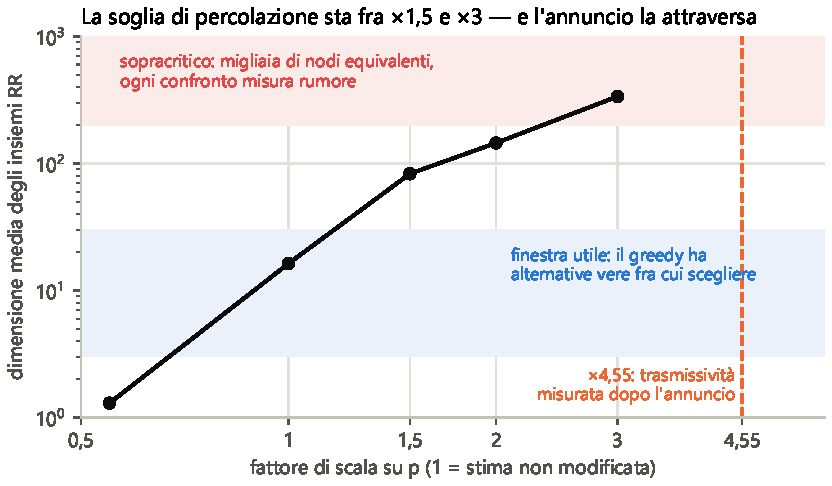
\includegraphics[width=\textwidth]{fig_regime}
    \caption{Dimensione degli insiemi RR contro il fattore di scala.}
    \label{fig:regime}
  \end{subfigure}\hfill
  \begin{subfigure}[t]{0.48\textwidth}
    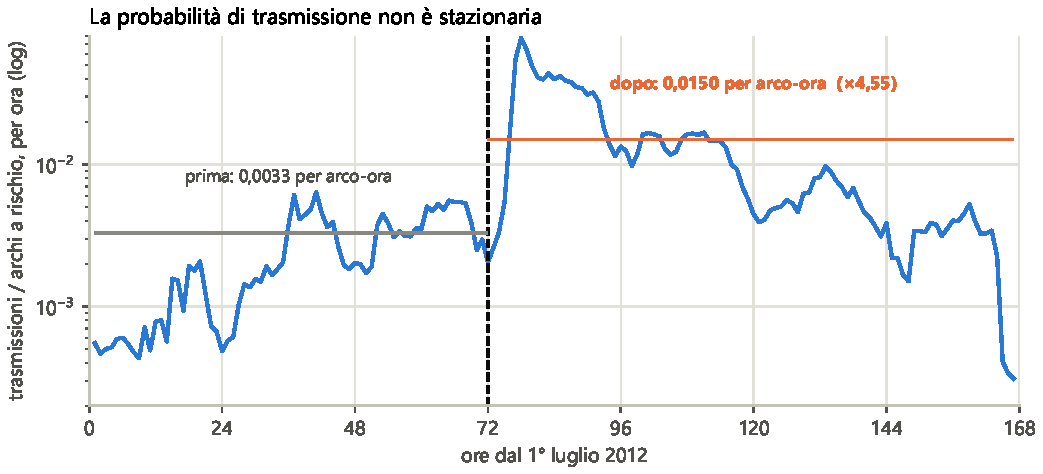
\includegraphics[width=\textwidth]{fig_stazionarieta}
    \caption{Il tasso di trasmissione per arco-ora.}
    \label{fig:stazionarieta}
  \end{subfigure}
  \caption{(a)~Alla scala 1 — la stima non modificata — il sistema è sottocritico e dentro la finestra utile; la soglia di percolazione sta fra $\times1{,}5$ e $\times3$. (b)~Dopo l'annuncio la trasmissività sale di 4,55 volte: la rete che nel periodo calmo non percola viene spinta oltre la soglia.}
\end{figure}
\paragraph{La stima estende bene, e non ha bisogno di essere frenata.} La credit distribution sui 28.498 archi ricchi dà una $p$ ben condizionata: mediana 0,0135, 99° percentile 0,2857, massimo 0,8276. Su \sx{} il 99° percentile della stima grezza era esattamente 1,0000, perché lì il numeratore era una coincidenza temporale fra adozioni e bastava una sola per saturare; qui è un retweet osservato, e la distribuzione lo riflette. La GNN estende la stima ai 14,8 milioni di archi poveri con MSE 0,000222 contro 0,001588 della costante: $-86\%$ (tabella~\ref{tab:gnn-archi}). Su \sx{} era $-48\%$.

La variante con la perdita pesata sul grado (l'ipotesi che l'MSE uniforme trascuri gli hub) peggiora l'MSE sugli hub del 2,1\%. Su \sx{} peggiorava del 2,0\%. Due substrati, stesso segno: è una replica indipendente, non un secondo tentativo sullo stesso dato, e l'ipotesi è respinta già sulla predizione, prima ancora dell'ablazione sui seed.

Con la $p$ della GNN usata così com'è, la dimensione media degli insiemi RR è 16,3 nodi sul campione ridotto usato per la taratura, e 29,0 sul campione pieno da 120.000 usato poi dalla Fase~3 (la distribuzione delle dimensioni ha coda pesante, pochi insiemi enormi pesano molto sulla media, e un campione di 1.200--1.500 insiemi la sottostima): in entrambi i casi dentro la finestra utile. Il fattore di regime scelto è quindi \textbf{1,00}: nessuna riscalatura. Su \sx{} la stima andava frenata a 0,25. È la seconda volta che la stessa misura dà esiti opposti sui due substrati, e la direzione è coerente: dove il numeratore è osservato, la stima è già nel regime giusto.

\paragraph{La soglia di percolazione, e l'annuncio che la attraversa.} La figura~\ref{fig:regime} colloca la soglia: a $\times1{,}5$ gli insiemi RR salgono a 83 nodi (critico), a $\times3$ a 336 (sopracritico). La figura~\ref{fig:stazionarieta} misura quanto la trasmissività cambia con l'annuncio: 0,0033 trasmissioni per arco-ora prima del confine, 0,0150 dopo, con il picco a 0,0398 all'ora 84. Fattore \textbf{4,55}, e sta oltre la soglia.

Le due misure insieme dicono una cosa che nessuna delle due dice da sola: nel periodo calmo la rete di Higgs \emph{non percola} (una cascata spontanea si spegne, e la $p$ stimata su quel periodo lo riflette correttamente), e l'annuncio del CERN, moltiplicando la trasmissività per 4,55, la spinge oltre il punto critico. L'esplosione dell'ora 76 non è arrivata dalla rete: è arrivata da fuori, e la rete l'ha amplificata perché lo shock l'ha portata sopra soglia. Questo è anche il motivo per cui la scelta dei seed si fa alla scala 1 e non a 4,55: sopra soglia migliaia di nodi sono equivalenti e il greedy sceglie fra pari a caso. Ma i seed scelti si possono \emph{valutare} a 4,55, ed è il controllo di \S\ref{sec:ris-validazione}.

\subsection{Fase 3: la superficie $k\times\alpha$}
\begin{figure}[htbp]
  \centering
  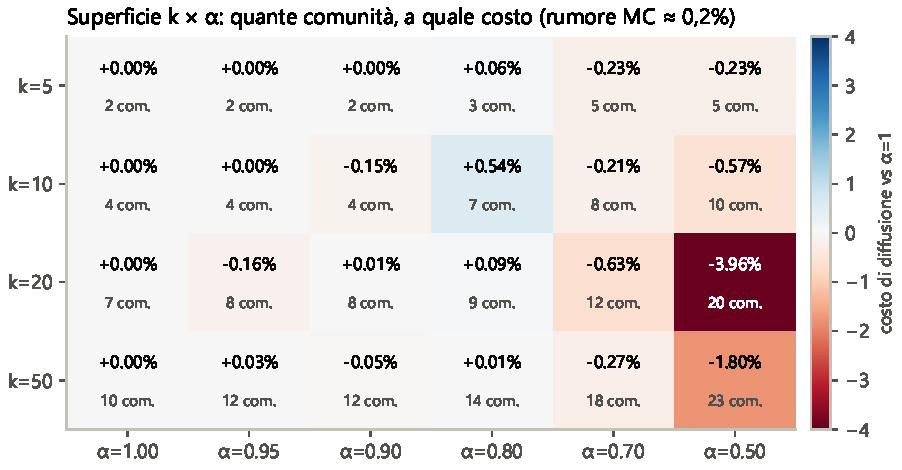
\includegraphics[width=0.85\textwidth]{fig_superficie}
  \caption{Costo di diffusione del vincolo di diversità rispetto a $\alpha=1$, e comunità toccate dai seed. Il rumore Monte Carlo sulla differenza fra due celle è circa lo 0,2\%.}
  \label{fig:superficie}
\end{figure}
\paragraph{Quante comunità, a quale costo.} Il rumore Monte Carlo di una singola stima di diffusione, misurato ripetendola con sei semi, è lo 0,12\% relativo a $k=50$ e lo 0,14\% a $k=10$; la differenza fra due celle della superficie ha quindi una deviazione standard di circa lo 0,2\%, e sotto quella soglia le celle non si distinguono. Con questo metro la figura~\ref{fig:superficie} si legge così. A $k=50$ TIM+ mette i cinquanta seed in dieci comunità; $\alpha = 0{,}80$ ne tocca quattordici a costo zero ($+0{,}01\%$, dentro il rumore), $\alpha = 0{,}70$ ne tocca diciotto per lo 0,27\% (poco più di una deviazione standard), $\alpha = 0{,}50$ le prende tutte e ventitré per l'1,80\%: l'unico punto in cui il prezzo si vede, e vale nove deviazioni standard. A $k=20$, da sette a nove comunità costa $+0{,}09\%$, cioè niente; a $k=10$, da quattro a sette comunità dà $+0{,}54\%$, che è 2,7 deviazioni standard \emph{sopra} zero: spargere i seed riduce la sovrapposizione fra le loro sfere d'influenza, e la diffusione sale.

Su \sx{} la stessa mossa a $k=5$ costava l'1,35\% e apriva comunità da due nodi. Qui il vincolo ha spazio per lavorare (ventitré comunità bilanciate) e il prezzo, dentro il modello, è quasi nullo. Se lo sia anche sul criterio esterno lo dice la sezione seguente.

\paragraph{L'ablazione della GNN, dentro il modello.} A regime pareggiato (23,6 nodi per insieme RR; scale 1,000 per la GNN, 0,539 per la costante) i seed scelti con la GNN diffondono 5.591,9 nodi attesi (la media, su 1.200 simulazioni, dei nodi attivati) sotto il modello della GNN contro 5.283,1 dei seed scelti con la costante ($+5{,}8\%$) e 5.380,0 del grado ($+3{,}9\%$). Sotto il modello costante la graduatoria si rovescia (20.539 contro 12.537): ogni modello preferisce i propri seed, e questo confronto è circolare per costruzione. I due pavimenti di rumore (43/50 per la costante contro sé stessa, 23/50 per la GNN contro sé stessa) e l'effetto di 14/50 dicono che i due modelli scelgono seed diversi più di quanto ciascuno differisca da sé; ma quale dei due scelga \emph{meglio} non può deciderlo nessuno dei due. Lo decide la validazione.

\subsection{La validazione: il punto di svolta}
\label{sec:ris-validazione}
\begin{figure}[htbp]
  \centering
  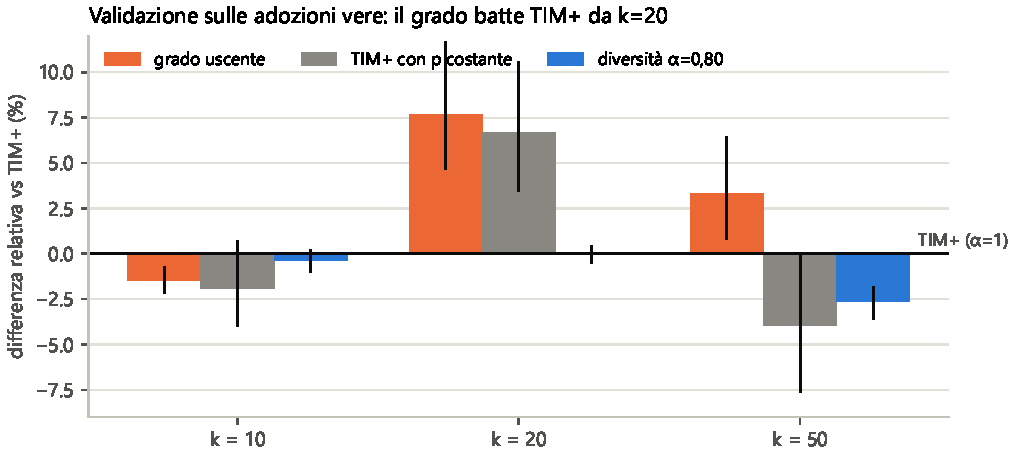
\includegraphics[width=0.9\textwidth]{fig_validazione}
  \caption{Differenza relativa dal TIM+ non pesato sul criterio esterno, con intervalli bootstrap. Il grado uscente batte TIM+ da $k=20$ in su; la $p$ costante non è coerentemente peggiore della GNN; il vincolo di diversità a $\alpha=0{,}80$ è gratis a $k=20$.}
  \label{fig:validazione}
\end{figure}

\begin{table}[htbp]
  \centering\small
  \caption{Validazione su adozioni vere: punteggio $\sum_v\pi(v)$ sui 269.081 adottanti, cioè il numero atteso di \emph{veri} adottanti che la cascata simulata dai seed raggiunge (178,3 a $k=50$: cinquanta seed raggiungono in media 178 dei 269.081). Differenza relativa dal riferimento TIM+ e $p$ del bootstrap a grappoli sull'ora. «A caso»: $k$ nodi estratti uniformemente; «solo fra i non attivi»: TIM+ con il divieto di scegliere chi ha già adottato.}
  \label{tab:validazione}
  \begin{tabular}{lrrr}
    \toprule
    strategia & $k=10$ & $k=20$ & $k=50$ \\
    \midrule
    TIM+ ($\alpha=1$), riferimento & 121,6 & 129,1 & 178,3 \\
    grado uscente & $-1{,}45\%$ ($p<0{,}001$) & $+7{,}66\%$ ($p<0{,}001$) & $+3{,}34\%$ ($p=0{,}001$) \\
    TIM+ con $p$ costante & $-1{,}91\%$ ($p=0{,}124$) & $+6{,}67\%$ ($p<0{,}001$) & $-3{,}94\%$ ($p=0{,}049$) \\
    diversità $\alpha=0{,}80$ & $-0{,}39\%$ ($p=0{,}216$) & $-0{,}02\%$ ($p=0{,}933$) & $-2{,}65\%$ ($p<0{,}001$) \\
    a caso & $-98{,}2\%$ & $-88{,}9\%$ & $-24{,}5\%$ \\
    solo fra i non attivi & $-80{,}8\%$ & $-70{,}8\%$ & $-58{,}6\%$ \\
    \bottomrule
  \end{tabular}
\end{table}
\paragraph{Il negativo, detto per primo.} Sul criterio esterno, la somma di $\pi(v)$ sui 269.081 utenti che hanno davvero adottato, \textbf{il grado uscente batte TIM+} a $k = 20$ ($+7{,}66\%$, $p < 0{,}001$) e a $k = 50$ ($+3{,}34\%$, $p = 0{,}001$), entrambi sotto la soglia di Bonferroni. Solo a $k = 10$ vince TIM+ ($-1{,}45\%$ per il grado, $p < 0{,}001$). Il risultato regge anche valutando gli stessi seed alla trasmissività misurata $\times 4{,}55$: a $k = 50$, $+2{,}25\%$ per il grado con $p < 0{,}001$. Credit distribution, GraphSAGE, RR-sketch e greedy con garanzia $1 - 1/e$ perdono contro «prendi i venti account con più follower».

Non è rumore, e non è che il modello non abbia segnale: batte la scelta casuale del 24\% a $k = 50$ e del 98\% a $k = 10$, e la scelta casuale fra i soli già attivi del 42\% e del 75\%. È che il grado è un predittore \emph{migliore} di chi adotterà. La ragione, che le sezioni seguenti confermano, è che TIM+ massimizza il \emph{numero} atteso di nodi attivati, e non sa quali di quei nodi sono i 269.081 che contano.

\paragraph{La GNN sugli archi non aiuta i seed.} Contro una $p$ costante portata allo stesso regime, la $p$ della GNN produce seed equivalenti a $k = 10$ ($p = 0{,}124$), \emph{peggiori} a $k = 20$ (la costante è avanti del 6,67\%, $p < 0{,}001$), e migliori a $k = 50$ ($+3{,}94\%$, ma $p = 0{,}049$, che non regge Bonferroni). Tre budget, tre risposte. Il modello che stima $p$ l'86\% meglio della costante non produce seed migliori: è la distinzione fra prevedere bene la trasmissione e decidere meglio da chi partire, e va scritta come un negativo.

\paragraph{Escludere chi è già attivo distrugge tutto.} Il vincolo realistico «non reclutare chi sta già parlando dell'evento» costa dal 58,6\% ($k = 50$) all'80,8\% ($k = 10$): i già attivi sono esattamente gli hub che il modello vorrebbe scegliere, e senza di loro il criterio esterno crolla. È un limite del criterio quanto della strategia: un già attivo scelto come seed si prende il merito di adozioni che sarebbero avvenute comunque.

\paragraph{Il potere esplicativo assoluto.} Partendo da \emph{tutti} i 35.610 utenti già attivi al confine (che non sono un budget ma il dato di fatto) il modello spiega 678 adozioni su 269.081: lo 0,3\%. Con cinquanta seed ne spiega 178. Un evento guidato da uno shock esogeno non è riproducibile da un Independent Cascade tarato sul periodo calmo che lo precede; il fattore 4,55 lo misura, ma il modello non lo contiene. I confronti fra strategie sono validi perché sono appaiati e relativi; i valori assoluti dicono quanto poco della cascata sta nel modello.

\paragraph{Il positivo: la diversità è gratis.} A $k = 20$ il vincolo con $\alpha = 0{,}80$ costa lo 0,02\% con $p = 0{,}933$, gratis in senso letterale, mentre porta i seed da sette a nove comunità. A $k = 10$, $-0{,}39\%$ con $p = 0{,}216$, equivalente. A $k = 50$ il costo si vede ($-2{,}65\%$, $p < 0{,}001$), ma alla trasmissività misurata $\times 4{,}55$ torna a sparire: $\alpha = 0{,}70$ dà $-0{,}24\%$ con $p = 0{,}343$ e apre diciotto comunità invece di dieci. La raccomandazione pratica che ne esce è precisa: il vincolo si usa, perché raddoppia le comunità raggiunte a un prezzo che sul criterio esterno non si distingue da zero.

\subsection{Chi adotterà: sette gradini}
\begin{figure}[htbp]
  \centering
  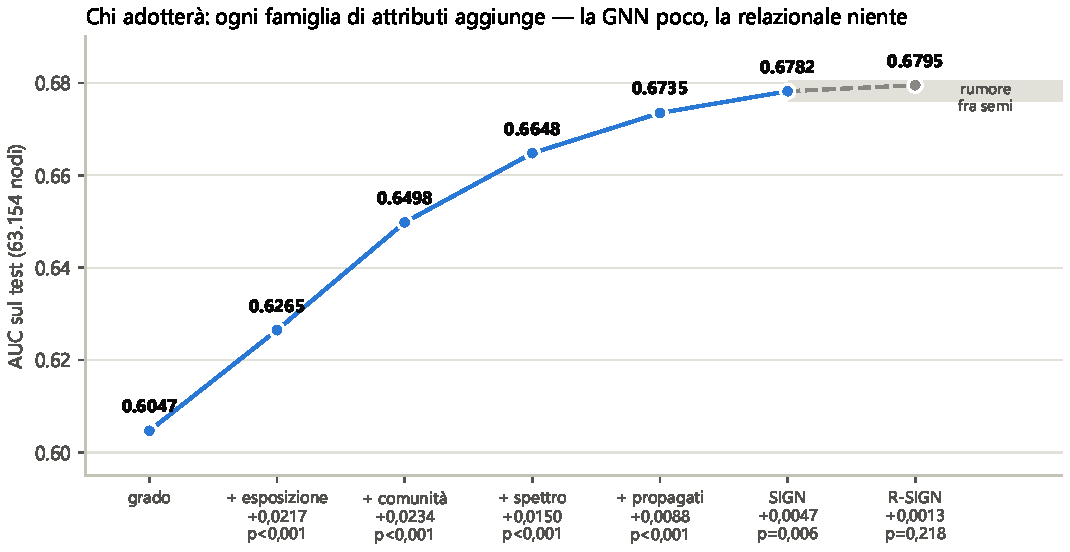
\includegraphics[width=\textwidth]{fig_scala}
  \caption{AUC sul test a ogni gradino, con il salto dal precedente e il suo $p$. Cinque salti positivi sotto Bonferroni; il sesto, verso R-SIGN, dentro il rumore fra semi.}
  \label{fig:scala}
\end{figure}

\begin{table}[htbp]
  \centering\small
  \caption{La scala a pioli. Bootstrap appaiato a grappoli sulle comunità, 2.000 repliche; Bonferroni su cinque confronti (soglia 0,010) per i primi cinque salti, su due (0,025) per il sesto.}
  \label{tab:scala}
  \begin{tabular}{lrrrrl}
    \toprule
    gradino & attr. & AUC & $\Delta$AUC & IC 95\% & $p$ \\
    \midrule
    grado & 2 & 0,6047 & — & — & — \\
    + esposizione & 6 & 0,6265 & $+0{,}0217$ & $[+0{,}0117,\,+0{,}0332]$ & $<0{,}001$ \\
    + comunità & 10 & 0,6498 & $\mathbf{+0{,}0234}$ & $[+0{,}0102,\,+0{,}0366]$ & $<0{,}001$ \\
    + spettro & 42 & 0,6648 & $+0{,}0150$ & $[+0{,}0091,\,+0{,}0242]$ & $<0{,}001$ \\
    + propagati & 126 & 0,6735 & $+0{,}0088$ & $[+0{,}0050,\,+0{,}0139]$ & $<0{,}001$ \\
    SIGN & 126 & \textbf{0,6782} & $+0{,}0047$ & $[+0{,}0015,\,+0{,}0085]$ & 0,006 \\
    \midrule
    + propagati relazionali (alberi) & 420 & 0,6767 & $+0{,}0031$ & $[+0{,}0012,\,+0{,}0052]$ & 0,006 \\
    R-SIGN & 420 & 0,6795 & $+0{,}0013$ & $[-0{,}0008,\,+0{,}0039]$ & 0,218 \\
    \midrule
    \emph{SIGN, altro seme} & & 0,6786 & $+0{,}0004$ & $[-0{,}0021,\,+0{,}0023]$ & 0,722 \\
    \emph{R-SIGN, altro seme} & & 0,6804 & $+0{,}0009$ & $[-0{,}0007,\,+0{,}0026]$ & 0,250 \\
    \bottomrule
  \end{tabular}
\end{table}
\paragraph{Cinque salti, cinque positivi.} Ogni famiglia di attributi aggiunge informazione sulla precedente, e ogni salto regge la correzione di Bonferroni: l'esposizione $+0{,}0217$, le comunità $+0{,}0234$, lo spettro $+0{,}0150$, la propagazione $+0{,}0088$, tutti con $p < 0{,}001$; la GNN $+0{,}0047$ con $p = 0{,}006$ contro una soglia di 0,010. È la prima scala di ablazioni interamente positiva del lavoro, ed è positiva sul criterio più severo che il protocollo prevede: bootstrap a grappoli sulle comunità, che sono l'unità di dipendenza più larga.

\paragraph{Le comunità sono il gradino più grande.} Il salto dall'esposizione alle comunità, $+0{,}0234$, supera quello dal grado all'esposizione. Sapere quanto è accesa la propria comunità e quanta della propria esposizione viene da dentro predice l'adozione più di sapere quanti dei propri seguiti sono attivi. È la community detection quantificata come informazione predittiva, con le comunità che entrano come numeri e non come identità: quindi non è memorizzazione di quale comunità adotta di più, è la struttura.

\paragraph{La GNN aggiunge poco, ma davvero.} Il salto da «propagati» a SIGN (stesso ingresso, MLP al posto degli alberi) vale $+0{,}0047$; il rumore fra due semi di SIGN è $+0{,}0004$ con intervallo $[-0{,}0021, +0{,}0023]$, quindi l'effetto lo supera di dieci volte. Ma va letto insieme al salto precedente: la propagazione precalcolata, data agli stessi alberi, aveva già preso $+0{,}0088$. L'aggregazione sul grafo conta; la non-linearità sopra conta la metà.

\paragraph{La struttura relazionale informa, ma la GNN non ne ha bisogno.} Gli attributi relazionali (direzione e tipo di relazione separati) dati agli stessi alberi aggiungono $+0{,}0031$ con $p = 0{,}006$, sotto Bonferroni (soglia 0,025): l'informazione c'è. Dati alla GNN, R-SIGN contro SIGN vale $+0{,}0013$ con $p = 0{,}218$, dentro il rumore fra semi ($+0{,}0009$). Il MLP sull'aggregazione simmetrica estrae già per via non lineare ciò che gli alberi ricavano solo se glielo si separa in ingresso. I pesi dei dieci blocchi in R-SIGN sono piatti, nessuna relazione domina, e i tre blocchi di interazione sono i più leggeri, coerente col fatto che entrano solo a due passi. È un risultato che dice dove un'informazione vera smette di servire.

\paragraph{Due cose sull'assoluto.} L'AUC finale, 0,678, è modesta: prevedere chi twitterà del bosone in quattro giorni dalla sola struttura pre-annuncio, senza contenuto e senza storia, è difficile, e il numero va presentato per quello che è. E la GraphSAGE a nodi end-to-end, che era la prima scelta, non era la strada: 95 secondi a epoca, 5,3 ore per 200 epoche, e un'AUC di validazione di 0,6666 ancora in salita. SIGN fa lo stesso lavoro in 92 secondi e arriva a 0,678.

\subsection{IM pesata dalla previsione}
\begin{figure}[htbp]
  \centering
  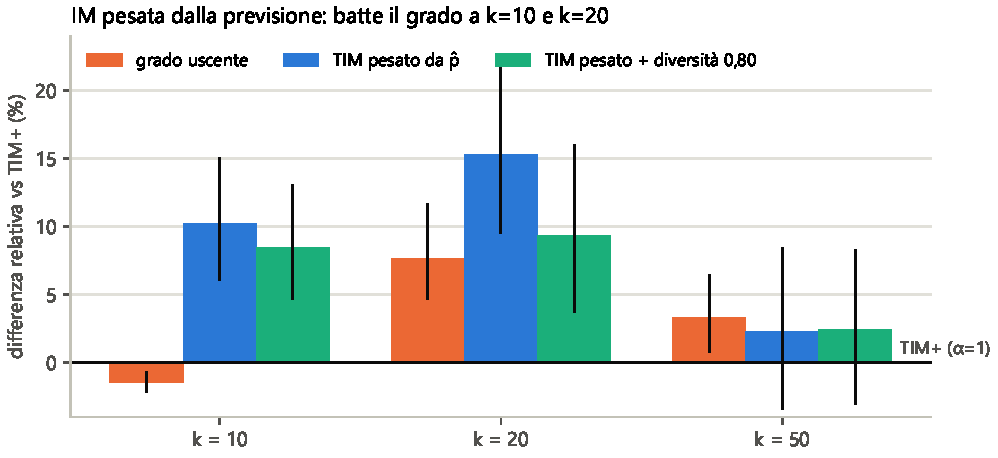
\includegraphics[width=0.9\textwidth]{fig_im_pesata}
  \caption{Differenza relativa dal TIM+ non pesato. Il TIM pesato da $\phat$ batte il grado a $k=10$ e $k=20$; a $k=50$ i tre sono equivalenti.}
  \label{fig:im-pesata}
\end{figure}

\begin{table}[htbp]
  \centering\small
  \caption{IM pesata: confronto diretto col grado uscente sul criterio esterno.}
  \label{tab:im-pesata}
  \begin{tabular}{lrrr}
    \toprule
    vs grado uscente & $k=10$ & $k=20$ & $k=50$ \\
    \midrule
    TIM+ non pesato & $+1{,}47\%$ & $-7{,}12\%$ & $-3{,}23\%$ \\
    TIM pesato da $\phat$ & $\mathbf{+11{,}85\%}$ ($p<0{,}001$) & $\mathbf{+7{,}06\%}$ ($p<0{,}001$) & $-1{,}01\%$ ($p=0{,}727$) \\
    TIM pesato + diversità 0,80 & $+10{,}05\%$ ($p<0{,}001$) & $+1{,}55\%$ ($p=0{,}516$) & $-0{,}85\%$ ($p=0{,}723$) \\
    seed già attivi (pesato) & 5/10 & 7/20 & 10/50 \\
    \bottomrule
  \end{tabular}
\end{table}
\paragraph{Dove il grado vinceva, ora perde.} Il TIM pesato dalla previsione out-of-fold batte il grado uscente dell'\textbf{11,85\%} a $k = 10$ (IC 95\% $[+9{,}1, +20{,}1]$) e del \textbf{7,06\%} a $k = 20$ ($[+4{,}0, +15{,}9]$), entrambi con $p < 0{,}001$ nel confronto diretto (tabella~\ref{tab:im-pesata}). A $k = 20$, proprio dove il grado batteva TIM+ di più, il pesato supera TIM+ del 15,26\%. Il risultato regge alla trasmissività misurata: valutati a $\times 4{,}55$, a $k = 20$ il pesato è avanti su TIM+ del 4,98\% contro il 3,17\% del grado. A $k = 50$ il vantaggio si esaurisce: pesato e grado sono equivalenti ($-1{,}01\%$, $p = 0{,}727$), coerente con tutto il resto: il vantaggio di qualunque modello sul grado si spegne quando il budget cresce.

\paragraph{Chi sceglie.} Il TIM pesato sceglie \emph{pochi seed già attivi}: 7 su 20, contro 20 su 20 di TIM+ e 19 su 20 del grado. Trova utenti che non parlano ancora dell'evento ma raggiungono chi adotterà: lo scenario realistico di una campagna, e l'opposto di ciò che il vincolo «solo fra i non attivi» faceva, perdendo l'80\%. La differenza è che qui i non attivi non sono imposti: sono scelti perché la previsione dice che i loro seguaci adotteranno.

\paragraph{Con la diversità sopra.} A $k = 20$, il TIM pesato con $\alpha = 0{,}80$ tocca venti comunità invece di cinque ed è alla pari col grado ($+1{,}55\%$, $p = 0{,}516$): tutte le comunità al prezzo del grado, non a meno. A $k = 10$ anche questa versione lo batte, del 10,05\%.

\paragraph{Che cosa dimostra.} Il classificatore ha un'AUC di 0,68, che nessuno chiamerebbe alta. Eppure basta a rovesciare il confronto: un ottimizzatore che sa \emph{un po'} chi adotterà batte sia l'ottimizzatore che non lo sa sia l'euristica che vinceva. La sofisticazione del modello di $p$ sugli archi non pagava sui seed (\S\ref{sec:ris-validazione}); la previsione sui nodi sì. È la distinzione fra sapere \emph{come} si trasmette e sapere \emph{a chi}.

% =====================================================================
\clearpage
\section{Discussione e limiti}
\label{sec:discussione}

I risultati del capitolo precedente contengono tanti negativi quanti positivi. Questo capitolo non li rivela (sono già scritti dove sono stati misurati) ma li interpreta, e dice che cosa il lavoro non può concludere.

\subsection{Perché il grado batte TIM+, e perché la previsione lo rovescia}
Il risultato più scomodo della relazione è che un'euristica di una riga batte una pipeline di tre fasi. Vale la pena capire perché, invece di spiegarlo via.

TIM+ massimizza $\sigma(S)$, il numero atteso di nodi attivati sotto il modello. Il criterio esterno non conta i nodi attivati: conta quelli, fra gli attivati, che hanno \emph{davvero} adottato. Le due quantità coincidono solo se ogni nodo ha la stessa probabilità di essere un vero adottante, e non è così: il classificatore della scala lo misura, con un'AUC di 0,68. TIM+ è quindi l'ottimo di una funzione obiettivo sbagliata di poco, e il grado, che concentra la copertura sugli hub e sui loro seguaci (dove la densità di veri adottanti è più alta, perché l'esposizione predice l'adozione), ci si avvicina meglio per caso. A $k = 10$ l'errore è piccolo e TIM+ vince ancora; a $k = 20$ e $k = 50$ i seed aggiuntivi di TIM+ vanno a coprire nodi che non adotteranno, e il grado passa avanti.

L'IM pesata corregge la funzione obiettivo, non l'ottimizzatore: le radici estratte in proporzione a $\phat(v)$ fanno sì che la copertura conti gli adottanti probabili, e lo stesso greedy con la stessa garanzia batte il grado dell'11,85\% e del 7,06\%. Il fatto che basti un'AUC di 0,68 dice che il peso non deve essere buono in assoluto: deve essere \emph{meglio dell'uniforme}, che è ciò che TIM+ assume. È la distinzione che il lavoro propone come tesi: sapere \emph{come} si trasmette, la $p$ sugli archi, dove la GNN è ottima, non aiuta a scegliere i seed; sapere \emph{a chi} (la $\phat$ sui nodi) sì.

Che il vantaggio si esaurisca a $k = 50$ è coerente: con cinquanta seed su una rete dove le comunità utilizzabili sono ventitré, ogni strategia ragionevole copre gli stessi hub, e la differenza sta nei seed marginali, dove il segnale della previsione è più debole.

\subsection{Che cosa non ha funzionato}
\begin{table}[htbp]
  \centering\small
  \caption{Le ablazioni negative, come sono state verificate.}
  \label{tab:negativi}
  \begin{tabular}{p{0.3\textwidth}p{0.62\textwidth}}
    \toprule
    componente & esito e verifica \\
    \midrule
    GNN sugli archi, per i seed & stima $p$ l'86\% meglio della costante, ma sul criterio esterno nessun vantaggio coerente: equivalenti a $k=10$, costante avanti a $k=20$, GNN avanti a $k=50$ con $p=0{,}049$ \\
    loss pesata sugli hub & respinta su entrambi i substrati: $-2{,}1\%$ e $-2{,}0\%$ \\
    aggregazione relazionale (R-SIGN) & la struttura informa gli alberi ($+0{,}0031$, $p=0{,}006$) ma non la GNN ($+0{,}0013$, $p=0{,}218$, dentro il rumore fra semi) \\
    esclusione dei già attivi dai seed & da $-58{,}6\%$ a $-80{,}8\%$: toglie esattamente chi conta \\
    M-EMCD (su \sx{}) & $\Qesp$ 0,0445 contro 0,1274 della fusione \\
    fusione multistrato convenzionale & $-0{,}1517$ di $\Qtras$, $p<0{,}001$ \\
    \bottomrule
  \end{tabular}
\end{table}

La tabella~\ref{tab:negativi} raccoglie le ablazioni negative con il modo in cui sono state verificate. Tre osservazioni le tengono insieme.

La prima è che i negativi \emph{si replicano}. La perdita pesata sugli hub è respinta con lo stesso segno su due substrati diversi; la GNN sugli archi stima bene e non sceglie meglio su tre budget diversi; la fusione convenzionale perde su \sx{} e su \hg{}. Un negativo che si ripete in condizioni indipendenti è un risultato, non un incidente.

La seconda è che alcuni negativi \emph{spiegano} altri risultati. Sulla popolazione da prevedere i gradi sugli strati di interazione sono identicamente zero, perché comparire in un retweet, in una mention o in una reply è esattamente ciò che definisce l'essere attivi. È una proprietà del dato, non un fallimento di una famiglia di attributi, e dice perché il multistrato entra nella previsione solo attraverso i vicini, e perché R-SIGN, che li vede a due passi, aggiunge poco. Che escludere i già attivi dai seed costi l'80\% dice che il criterio esterno premia chi si prende il merito di adozioni già in corso, ed è la ragione per cui il risultato dell'IM pesata, che sceglie pochi già attivi \emph{e} batte il grado, è più forte di quanto il numero da solo dica.

La terza è che il negativo più importante, il grado che batte TIM+, è stato il punto di svolta del lavoro e non la sua fine. La sezione precedente dice perché.

\subsection{Il potere esplicativo assoluto}
Partendo da tutti i 35.610 utenti già attivi al confine, il modello di diffusione spiega 678 adozioni su 269.081: lo 0,3\%. Il numero va letto insieme al fattore di non stazionarietà: la $p$ è stimata sul periodo calmo, dove la rete è sottocritica e una cascata si spegne dopo pochi passi, e nel periodo di verifica la trasmissività è 4,55 volte maggiore e la rete è sopra soglia. Un Independent Cascade tarato sul primo periodo non può riprodurre il secondo, per costruzione.

Questo non invalida i confronti fra strategie, che sono appaiati e relativi, e che il controllo a $\times 4{,}55$ conferma. Ma delimita ciò che il lavoro può dire: misura quale strategia \emph{indirizza meglio} verso i veri adottanti, non quanto della cascata la rete spieghi. La cascata di Higgs è stata innescata da un evento esterno che ha raggiunto tutti contemporaneamente, e il modello lo sa solo nella misura in cui lo misura (il fattore 4,55), senza contenerlo. Modellare lo shock, con una $p$ che dipenda dal tempo o con un termine di attivazione esogena, è la prima cosa che il lavoro non fa.

\subsection{Limiti del dato}
\emph{Il grafo dei follower è stato raccolto attorno all'evento.} Gli archi di follow non hanno data, e una parte di essi può essere nata durante l'esplosione. In quel caso una frazione della struttura che i modelli usano per prevedere sarebbe una conseguenza di ciò che prevedono. L'effetto, se c'è, va nella direzione di gonfiare tutti i risultati che usano il grafo (il cancello, $\Qtras$, l'esposizione, la scala) e non è correggibile con i dati disponibili. Il fatto che il cancello dia zero su \sx{}, dove il problema non si pone, è l'unica garanzia che il protocollo non produca eccesso strutturale dal nulla.

\emph{Un evento solo.} Tutti i bootstrap di \hg{} ricampionano unità dentro lo stesso evento (ore, comunità), mai eventi diversi. Gli intervalli dicono quanto i risultati sono stabili \emph{su questa cascata}, non quanto generalizzino a un'altra. \sx{} è l'unico secondo caso, ed è un controllo negativo, non una replica.

\emph{Nessun identificativo di cascata.} Il log dice chi ha ritwittato chi, ma non quale tweet: non si possono ricostruire le cascate come alberi, e la previsione della dimensione di una cascata, il problema standard della letteratura, non è possibile su questo dato. La domanda del lavoro, «chi adotterà», è quella che il dato permette di porre.

\emph{Non tutte le trasmissioni passano per il grafo di follow.} Una parte dei retweet osservati avviene fra utenti non collegati da un arco di follow, attraverso timeline altrui, ricerca o trend. Il grafo dei follower resta il canale principale e l'unico osservabile prima dell'evento, ma la quota di diffusione che scorre fuori da esso non è modellata.

\subsection{Limiti del metodo}
\emph{L'AUC finale è 0,68.} Ogni gradino aggiunge in modo significativo, ma il totale resta modesto: prevedere chi twitterà del bosone in quattro giorni dalla sola struttura pre-annuncio, senza contenuto, senza storia degli utenti e senza il testo dei tweet, è difficile, e il lavoro non lo nasconde. Il valore della scala sta nelle \emph{differenze} fra gradini, che sono la misura dell'informazione di ogni famiglia; il valore assoluto dice quanto la struttura da sola può fare.

\emph{Un R-GCN vero non è stato addestrato.} R-SIGN è il primo strato di un R-GCN senza la non-linearità fra le aggregazioni; un R-GCN a batch pieno su 456.627 nodi non è praticabile su CPU, e una versione a campionamento di vicinato è stata giudicata fuori perimetro. È possibile che un R-GCN completo estragga dalla struttura relazionale più di quanto R-SIGN faccia; il lavoro può dire solo che, al primo strato, la GNN non ne ha bisogno.

\emph{Iperparametri fissi.} Nessun modello è stato tarato per gradino, di proposito: la domanda è quale famiglia porta informazione, e una ricerca per gradino confonderebbe attributi migliori con modelli tarati meglio. Il prezzo è che ogni AUC è probabilmente sottostimata di qualche millesimo, in modo uniforme.

\emph{Le comunità come numeri.} Le comunità entrano nella previsione come dimensione, quota accesa ed esposizione interna, mai come identità categorica. È una scelta, l'identità non generalizza, e non è ciò che si vuole misurare, che esclude per costruzione un possibile guadagno: se alcune comunità adottano più di altre per ragioni che i numeri non catturano, la scala non lo vede.

\emph{Il criterio esterno usa $\pi$ del modello.} Il punteggio di validazione somma probabilità di attivazione \emph{stimate}, sui veri adottanti: misura quanto il modello indirizza verso di loro, ed è dipendente dalla $p$ e dalla scala. Il controllo a $\times 4{,}55$ mostra che la graduatoria regge cambiando scala, ma un criterio del tutto indipendente dal modello (per esempio la quota di veri adottanti raggiunti in $h$ passi lungo il grafo) non è stato usato.

% =====================================================================
\clearpage
\section{Conclusioni}
\label{sec:conclusioni}
Il lavoro è partito da una domanda di ottimizzazione, da chi partire per diffondere il più possibile toccando più comunità possibile, e arriva a due tesi che non erano nel progetto iniziale. Nessuna delle due è stata cercata: entrambe sono emerse da misure che hanno dato esiti diversi da quelli sperati, e dalla decisione di seguirle.

\paragraph{Il substrato decide, e si può sapere prima.} L'eccesso strutturale stratificato contro un modello nullo a gradi preservati si misura in mezza giornata, prima di scrivere una riga di pipeline, e predice se quella pipeline avrà qualcosa da trovare. Su \sx{} vale zero, e infatti ogni componente lì è risultata nulla: non per difetti di implementazione, ma perché non c'era struttura da trovare. Su \hg{} vale $+73\%$, e le stesse componenti danno segnale. La soglia era stata fissata prima, e il verdetto è arrivato in entrambe le direzioni. \sx{} non è un fallimento da giustificare: è il controllo negativo che dimostra che il protocollo sa dire di no, e una pipeline che producesse risultati positivi su entrambi i substrati sarebbe meno credibile, non di più.

\paragraph{Prevedere prima di ottimizzare.} Anche sul substrato buono, l'ottimizzatore che massimizza \emph{quanti} nodi attiva perde contro l'euristica del grado, perché non sa \emph{quali} di quei nodi adotteranno. Un classificatore che lo sa un po' (un'AUC di 0,68, costruita per gradini in modo che ogni famiglia di attributi sia un'ablazione, con le comunità come famiglia più informativa) basta a rovesciare il confronto: lo stesso greedy, con le radici pesate dalla previsione, batte il grado. La sofisticazione del modello di trasmissione sugli archi non ha pagato sui seed; la previsione sui nodi sì. È la distinzione fra sapere come si trasmette e sapere a chi, e il lavoro la propone come regola: prima si prevede, poi si ottimizza sulla previsione.

Accanto alle tesi stanno i limiti, che il capitolo~\ref{sec:discussione} ha elencato e che qui si ripetono in una riga ciascuno: un evento solo; un grafo dei follower raccolto attorno all'evento; un modello di diffusione che spiega lo 0,3\% della cascata, perché lo shock che l'ha innescata è esterno e il modello lo misura senza contenerlo; un'AUC modesta; un R-GCN completo non addestrato.

\paragraph{Che cosa porterebbe avanti il lavoro.} Tre cose, in ordine di quanto cambierebbero le conclusioni. La prima è un \emph{secondo evento}, su una rete raccolta prima e non attorno: direbbe se l'eccesso strutturale e la scala a pioli generalizzano oltre questa cascata, e chiuderebbe il limite più serio del dato. La seconda è una \emph{cascata endogena}, non innescata da uno shock esterno: lì il modello di diffusione tarato sul periodo calmo dovrebbe spiegare molto più dello 0,3\%, e il confronto fra ottimizzatore e grado si farebbe in un regime in cui la rete conta davvero per la dinamica, non solo per la struttura. La terza è portare la previsione \emph{dentro} il modello di diffusione invece che accanto: usare $\phat(v)$ non come peso delle radici ma come probabilità di attivazione del nodo dentro l'Independent Cascade, o come termine di attivazione esogena che modelli lo shock. Sarebbe il passo che il fattore 4,55 chiede e che questo lavoro ha solo misurato.

Il risultato che resta, al di là dei numeri, è un protocollo: un cancello deciso prima, un criterio esterno, bootstrap appaiati sull'unità di dipendenza giusta, il rumore di riferimento accanto a ogni effetto, e i negativi scritti dove sono stati misurati. È ciò che ha permesso di cambiare domanda senza cambiare progetto, e di sapere, a ogni passo, se il numero sulla pagina era un risultato o un artefatto.

% =====================================================================
\appendix
\clearpage
\section{Tabelle complete}
\label{app:tabelle}
Le tabelle del capitolo~\ref{sec:risultati} sono estratte dalle uscite testuali di ogni esperimento, che stanno nel repository, con un file per esecuzione. Qui si riportano le tre che la relazione cita solo in parte.

\paragraph{La superficie $k \times \alpha$ completa.} Partizione «fusione calibrata», 1.200 simulazioni per cella, rumore Monte Carlo sulla singola stima 0,12--0,14\% relativo.
\begin{center}\small
\begin{tabular}{rrrrr@{\qquad}rrrrr}
\toprule
$k$ & $\alpha$ & com. & diffusione & costo & $k$ & $\alpha$ & com. & diffusione & costo \\
\midrule
 5 & 1,00 &  2 & 4.619,4 & —      & 20 & 1,00 &  7 & 5.038,6 & — \\
 5 & 0,95 &  2 & 4.619,4 & $0{,}00$ & 20 & 0,95 &  8 & 5.030,4 & $-0{,}16$ \\
 5 & 0,90 &  2 & 4.619,4 & $0{,}00$ & 20 & 0,90 &  8 & 5.039,1 & $+0{,}01$ \\
 5 & 0,80 &  3 & 4.622,3 & $+0{,}06$ & 20 & 0,80 & 9 & 5.043,1 & $+0{,}09$ \\
 5 & 0,70 &  5 & 4.608,9 & $-0{,}23$ & 20 & 0,70 & 12 & 5.007,0 & $-0{,}63$ \\
 5 & 0,50 &  5 & 4.608,9 & $-0{,}23$ & 20 & 0,50 & 20 & 4.839,1 & $-3{,}96$ \\
\midrule
10 & 1,00 &  4 & 4.767,3 & —      & 50 & 1,00 & 10 & 5.591,9 & — \\
10 & 0,95 &  4 & 4.767,3 & $0{,}00$ & 50 & 0,95 & 12 & 5.593,6 & $+0{,}03$ \\
10 & 0,90 &  4 & 4.760,4 & $-0{,}15$ & 50 & 0,90 & 12 & 5.589,0 & $-0{,}05$ \\
10 & 0,80 &  7 & 4.793,1 & $+0{,}54$ & 50 & 0,80 & 14 & 5.592,2 & $+0{,}01$ \\
10 & 0,70 &  8 & 4.757,4 & $-0{,}21$ & 50 & 0,70 & 18 & 5.576,7 & $-0{,}27$ \\
10 & 0,50 & 10 & 4.740,2 & $-0{,}57$ & 50 & 0,50 & 23 & 5.491,2 & $-1{,}80$ \\
\bottomrule
\end{tabular}
\end{center}
Il costo è in percento rispetto ad $\alpha = 1$; $\alpha = 0{,}30$ coincide ovunque con $\alpha = 0{,}50$, come la formula del tasso di scambio prevede.

\paragraph{La validazione completa a $k=50$, con intervalli.} Riferimento TIM+ ($\alpha = 1$), punteggio 178,3; bootstrap appaiato sull'ora, 3.000 repliche; soglia di Bonferroni 0,0050.
\begin{center}\small
\begin{tabular}{lrrrl}
\toprule
strategia & punteggio & differenza & IC 95\% & $p$ \\
\midrule
diversità $\alpha=0{,}90$ & 173,5 & $-2{,}68\%$ & $[-6{,}5,\,-3{,}3]$ & $<0{,}001$ \\
diversità $\alpha=0{,}80$ & 173,6 & $-2{,}65\%$ & $[-6{,}4,\,-3{,}3]$ & $<0{,}001$ \\
diversità $\alpha=0{,}70$ & 174,6 & $-2{,}07\%$ & $[-6{,}7,\,-0{,}2]$ & 0,045 \\
diversità $\alpha=0{,}50$ & 168,5 & $-5{,}49\%$ & $[-14{,}8,\,-5{,}1]$ & $<0{,}001$ \\
TIM+ fra i non attivi & 73,8 & $-58{,}59\%$ & $[-135{,}2,\,-78{,}2]$ & $<0{,}001$ \\
diversità fra i non attivi & 75,8 & $-57{,}46\%$ & $[-131{,}8,\,-77{,}5]$ & $<0{,}001$ \\
TIM+ con $p$ costante & 171,3 & $-3{,}94\%$ & $[-13{,}5,\,-0{,}1]$ & 0,049 \\
grado uscente & 184,2 & $+3{,}34\%$ & $[+1{,}5,\,+11{,}4]$ & 0,001 \\
a caso & 134,7 & $-24{,}46\%$ & $[-61{,}4,\,-27{,}6]$ & $<0{,}001$ \\
a caso fra gli attivi & 103,3 & $-42{,}07\%$ & $[-97{,}9,\,-55{,}2]$ & $<0{,}001$ \\
\bottomrule
\end{tabular}
\end{center}
Gli intervalli sono sulla differenza assoluta di punteggio. Alla trasmissività misurata $\times 4{,}55$ (150 simulazioni) il riferimento sale a 2.028,0; il grado resta avanti del 2,25\% ($p < 0{,}001$), $\alpha = 0{,}70$ scende a $-0{,}24\%$ ($p = 0{,}343$) e $\alpha = 0{,}90$ a $-0{,}50\%$ ($p = 0{,}103$).

\paragraph{I pesi dei blocchi in R-SIGN.} Norma di Frobenius di ciascuna $W_r$ sugli attributi standardizzati, seme 11: $x$ 3,29; $A_{\mathrm{in}}x$ 3,42; $A_{\mathrm{out}}x$ 3,51; $A_{\mathrm{in}}A_{\mathrm{in}}x$ 3,52; $A_{\mathrm{in}}A_{\mathrm{out}}x$ 3,59; $A_{\mathrm{out}}A_{\mathrm{in}}x$ 3,37; $A_{\mathrm{out}}A_{\mathrm{out}}x$ 3,48; $A_{\mathrm{in}}A_{\mathrm{RT}}x$ 3,18; $A_{\mathrm{in}}A_{\mathrm{MT}}x$ 3,10; $A_{\mathrm{in}}A_{\mathrm{RE}}x$ 3,21. Nessun blocco domina; i tre di interazione sono i più leggeri. È un indizio, non una prova.

\clearpage
\section{Il primo progetto su StackExchange}
\label{app:stackexchange}
La pipeline è stata eseguita per intero su \sx{} prima del cancello, con lo stesso protocollo. I numeri sono qui per due ragioni: sono il controllo negativo, e mostrano che cosa produce il protocollo su un substrato senza struttura, non risultati falsi, ma risultati nulli riconoscibili come tali.

\paragraph{Fase 1.} Cinque candidate su 46.312 nodi: Louvain su L1 (8.519 comunità), su L2 (8.319), sulla fusione L1+L2 (176), M-EMCD a $\theta = 0{,}4$ (3.086) e $\theta = 0{,}5$ (36.483), più il controllo a singoletti. Criterio decisionale $\Qesp$, la modularità sulla rete di esposizione dei 105 tag bersaglio (64.711 esposizioni); criterio tematico l'AMI col tag dominante degli utenti, disponibile per il 10\% dei nodi. La fusione vince con $\Qesp = 0{,}1274$ contro 0,1227 di L2, 0,0843 di L1, 0,0445 e 0,0104 di M-EMCD; il margine su L2 ha $p = 0{,}040$ nel bootstrap sui tag e \emph{non regge Bonferroni} (soglia 0,0125). M-EMCD a $\theta = 0{,}5$ produce quasi tutti singoletti: NMI 0,7185, AMI 0,0192, rapporto intra/caso 20,69$\times$: la riga da cui il lavoro ha imparato a diffidare delle metriche non corrette. Il controllo a singoletti prende NMI 0,7689 e AMI 0,0000. Sul sito piccolo, Computer Graphics, la fusione vince nettamente ($p = 0{,}008$, regge Bonferroni): il multistrato pagava dove un livello solo non aveva abbastanza dati.

\paragraph{Fase 2.} Credit distribution su adozioni di tag: il 47,9\% degli archi con dati, e un 99° percentile della $p$ grezza esattamente a 1,000, portato a 0,408 dallo smoothing. Il regime va frenato a 0,25 (insiemi RR da 225,9 nodi alla scala 1, 12,2 alla scala 0,25). La GraphSAGE sugli archi, dopo la correzione del bias d'uscita, batte la costante del 48\% di MSE; la perdita pesata sugli hub peggiora del 2,0\% su Security e migliora del 6,1\% su Computer Graphics.

\paragraph{Fase 3.} Pavimento di rumore 2/50, effetto della GNN 1/50: dentro il rumore. Diffusione attesa 563,9 con i seed della GNN contro 569,1 con quelli della costante e 510,1 col grado. Superficie $k \times \alpha$: a $k = 5$ TIM+ mette tutti e cinque i seed in una comunità sola, spargerli su cinque costa l'1,35\%; a $k \ge 20$ il costo è nullo perché il greedy li avrebbe sparsi comunque. Delle 176 comunità, 18 coprono il 99,2\% dei nodi; il vincolo senza soglia apriva gruppetti da due nodi.

\paragraph{Validazione.} Seed scelti con dati fino al 2019, adottanti veri 2020--2022, bootstrap sui 105 tag. TIM+ 648,3; $\alpha = 0{,}80$ $-0{,}42\%$ ($p < 0{,}001$); grado $-1{,}44\%$ ($p < 0{,}001$); casuale $-18{,}91\%$. Il 71,5\% degli adottanti reali era irraggiungibile perché iscritto dopo il confine. Il vantaggio di TIM+ sul grado passa da $+1{,}76\%$ nella prima metà dei tag a $+1{,}20\%$ nella seconda, e regge sotto tre ponderazioni diverse dell'attività mensile, che nella finestra scende da 889 a 467 utenti.

\paragraph{L'esperimento competitivo.} Due agenti con budget 5 su NetMax, turni alternati, ruoli scambiati, quota come metrica. Sul sito piccolo con trenta partite per configurazione, riferimento 46,1\% $\pm$ 3,5, nessuna variante di diversità oltre due errori standard. Sul sito grande con sei partite, errori di 10--18 punti: sottodimensionato, e riportato come tale.

\paragraph{La diagnosi.} Tutti questi effetti sono piccoli (frazioni di punto, $p$ al limite, ablazioni dentro il rumore) e all'epoca sembravano difetti di implementazione da correggere uno per uno. L'eccesso strutturale stratificato ($-0\%$) dice invece che erano il risultato giusto: su un substrato in cui la topologia non porta la diffusione, un protocollo onesto deve misurare quasi niente, e lo ha fatto.

\clearpage
\bibliographystyle{plainnat}
\bibliography{bibliografia}

\end{document}
